% !TeX program = pdflatex
\documentclass{iutbscthesis}
\usepackage{algorithm}
\usepackage{algpseudocode}

% The iutbscthesis uses biblatex for bibliography management.
\addbibresource{citations.bib}

% The complete title of your thesis, mandatory
\title{Tri-Level Calibration and Discriminative Prompt-Based Recalibration for Training-Free Few-Shot Class-Incremental Learning}

% Use the \addauthor command to keep adding authors with student ID
% TODO: replace with the real author name(s) and student ID(s) before printing.
\addauthor{Md Akib Haider}{XXXXXXXXX}

% Use the \supervisor command to define the supervisor with name, designation, and department
% TODO: replace with the real supervisor's name and designation before printing.
\supervisor{[Reaz Hassan Joarder]}{[Junior Lecturer]}{Department of Computer Science and Engineering}

% Complete department name, mandatory
\department{Department of Computer Science and Engineering}

% Complete program name, mandatory
\program{BACHELOR OF SCIENCE IN COMPUTER SCIENCE AND ENGINEERING}

% Date (day, month name, and year) when the presentation took place, mandatory
% TODO: replace with the real defense date.
\defensedate{15}{December}{2026}

\begin{document}

%-------------------------- FRONT MATTER --------------------------%

\coverpage

\pagenumbering{roman}

\titlepage

\declarationofcandidate

\dedicatedto{our families and teachers, whose patience and encouragement made this work possible}

\tableofcontents
\listoffigures
\listoftables

\clearpage

\begin{abbreviations}
    \abbr{FSCIL}{Few-Shot Class-Incremental Learning}
    \abbr{VLM}{Vision-Language Model}
    \abbr{CLIP}{Contrastive Language-Image Pre-training}
    \abbr{ViT}{Vision Transformer}
    \abbr{DINO}{Self-Distillation with No Labels}
    \abbr{LLM}{Large Language Model}
    \abbr{BiMC}{Bi-level Modality Calibration}
    \abbr{TRIC}{Tri-Level Calibration}
    \abbr{QPR}{Query Prototype Rectification}
    \abbr{DPR}{Discriminative Prompt-based Recalibration}
    \abbr{PD}{Performance Degradation}
    \abbr{CUB}{Caltech-UCSD Birds}
\end{abbreviations}

\begin{acknowledgement}

We would like to express our sincere gratitude to our supervisor for the guidance, patience, and constructive criticism that shaped every stage of this work, from the earliest reading of the few-shot class-incremental learning literature to the final wording of this report.

We are also thankful to the Department of Computer Science and Engineering, Islamic University of Technology, for providing the academic environment and resources necessary to pursue this research, and to our peers for many useful discussions on calibration, prompting, and evaluation practice in few-shot learning.

Finally, we thank our families for their unwavering support and understanding throughout the duration of this thesis.

\end{acknowledgement}

\begin{abstract}
Few-shot class-incremental learning (FSCIL) requires a system to learn a long stream of new classes from only a handful of labeled images per class while retaining accuracy on a much larger set of base classes learned earlier, and it must do so without revisiting old data. Recent training-free methods sidestep catastrophic forgetting altogether by keeping every encoder frozen and assembling the final classifier from pre-computed prototypes, but this convenience exposes two problems that jointly calibrated pipelines built on a single vision-language backbone cannot solve: a self-supervised visual encoder such as DINOv2 lives in a geometrically incompatible embedding space from a vision-language encoder such as CLIP, so the two cannot simply be averaged; and every novel-class prototype is estimated from as few as five images, leaving it too noisy to trust without further evidence. This thesis studies both problems together. First, we adopt and explain in full pedagogical detail Tri-Level Calibration (TRIC), a training-free framework that resolves the incompatibility problem by separating the assembly of the final classifier into three explicit calibration steps: a semantic calibration inside the language branch, an inter-model calibration that fuses CLIP and DINOv2 visual evidence on a common class-score axis rather than in raw embedding space, and an inter-modal calibration that fuses the resulting semantic and visual evidence. On top of this calibrated backbone, we describe Query Prototype Rectification (QPR), a label-free module that uses the unlabeled query batch arriving in every session to refine only the noisy novel-class visual prototypes, admitting a query for refinement only when the calibrated posterior itself is confident that the query belongs to a novel class. Second, and as the principal extension proposed in this thesis, we design Discriminative Prompt-based Recalibration (DPR), a further, purely label-only refinement of the semantic branch that identifies pairs of classes whose prototypes are too similar, generates prompts that linguistically contrast each such pair, and uses an iterative, safeguarded update rule to sharpen the separation between confusable classes without degrading their separation from every other class. We report and analyze the published evaluation of TRIC and TRIC-QPR across three standard FSCIL benchmarks, miniImageNet, CIFAR-100, and CUB-200, where the tri-level backbone improves final-session accuracy over the strongest training-free baseline by 9.83, 1.32, and 12.53 points respectively, and the label-free rectification stage adds a further 2.43, 1.01, and 0.88 points with a positive gain in every evaluated random seed. We further present a complete algorithmic specification of DPR, a worked illustrative example of its recalibration procedure, and a concrete case study, drawn from the fine-grained CUB-200 benchmark, that motivates exactly the failure mode DPR is designed to address, together with a proposed protocol for its empirical validation as future work.
\end{abstract}

%-------------------------- MAIN BODY --------------------------%
\pagenumbering{arabic}

\chapter{Introduction}
\label{chapter:introduction}

\section{Background and Motivation}

Standard image classifiers are trained once, on a fixed set of classes, under the assumption that the world they will be deployed into looks like the world they were trained on. Real deployments rarely honor that assumption: new categories of interest appear after deployment, and in many practically important settings---rare wildlife species, newly registered products in a catalogue, previously unseen defect types on a production line---only a handful of labeled examples of each new category are ever going to be available. \emph{Few-shot class-incremental learning} (FSCIL) formalizes this setting \autocite{tao2020fewshot}. A model is first trained on a base session with many labeled examples per class, and is then exposed to a sequence of incremental sessions, each introducing a small number of brand-new classes with only $K$ labeled images per class (typically $K=5$). After every session, the model must correctly classify a held-out query batch drawn from every class seen so far, including the original base classes. Crucially, the model is not allowed to revisit the training images of earlier sessions, so it must accumulate new knowledge while retaining old knowledge under a hard memory constraint.

This combination of constraints creates a well-known tension in continual learning: adapting a model's parameters to fit new, scarce data tends to overwrite the representations that were previously useful for old, plentiful data, a phenomenon usually called \emph{catastrophic forgetting} \autocite{parisi2019continual, delange2021continual}. FSCIL adds a second difficulty on top of forgetting: because each new class is supported by only a handful of images, whatever a model learns about a new class is itself built on a small and potentially unrepresentative sample, so incremental learning here is also a few-shot learning problem \autocite{chen2019closer, snell2017prototypical, vinyals2016matching, finn2017modelagnostic}.

A large body of FSCIL research addresses forgetting by carefully controlling how a model's trainable parameters are updated across sessions: by replaying or regularizing against previously learned representations \autocite{rebuffi2017icarl, li2016learning}, by evolving a lightweight classifier incrementally while freezing a shared backbone \autocite{zhang2021continually}, by distilling semantic structure from a teacher into the incremental representation \autocite{cheraghian2021semantic}, by shaping the base-session representation so that it is already ``forward compatible'' with classes that have not been observed yet \autocite{zhou2022forward}, by meta-learning an update rule that generalizes across sessions \autocite{chi2022metafscil}, or by regularizing the geometry of the learned class prototypes \autocite{zhao2023classaware}. These trainable approaches are effective, but they still require some form of gradient-based adaptation at every incremental session, which reintroduces exactly the risk of forgetting they are designed to control, and which is often costly to run at deployment time.

An alternative line of work removes incremental training altogether. \emph{Training-free} FSCIL methods keep every network weight frozen after base-session pre-training (or use an off-the-shelf frozen foundation model from the outset) and construct the classifier for each new session purely by computing and combining prototypes---typically the mean of the frozen feature vectors of each class's support images---with no gradient update at all \autocite{wang2023teen, goswami2023fecam, chen2025bimc}. Because nothing in the backbone ever changes, catastrophic forgetting of the base classes is structurally impossible; the only question is how to assemble accurate class prototypes, and how to combine them into a classifier, using only frozen evidence. Recent training-free methods lean heavily on large vision-language models such as CLIP \autocite{radford2021learning}, which pair a frozen image encoder with a frozen text encoder trained so that an image and a matching natural-language description land near each other in a shared embedding space. This makes it possible to build not just a visual prototype for each class from its few support images, but also a \emph{semantic} prototype directly from the class name or a short natural-language description of the class, with no images at all. The BiMC framework \autocite{chen2025bimc} formalizes the resulting design space as \emph{bi-level modality calibration}: a CLIP semantic prototype, enriched with class descriptions, is combined with a CLIP visual prototype through a soft base-prototype shift, and the two are then fused with auxiliary evidence at the logit level.

This bi-level view is internally consistent as long as every piece of visual evidence comes from the same encoder. It stops being consistent the moment a second, structurally different visual encoder is introduced. Self-supervised visual encoders such as DINO and DINOv2 \autocite{caron2021emerging, oquab2023dinov2} are trained with an entirely different objective from CLIP---image-level self-distillation rather than image-text contrastive alignment---and they are known to produce markedly different embedding geometry: CLIP's image branch is trained to align with text and tends to produce visually dense class prototypes, whereas DINOv2 is trained purely for visual self-similarity and produces much sparser, more separable prototypes. Averaging a CLIP prototype and a DINOv2 prototype directly, as a naive extension of the bi-level view would suggest, is geometrically meaningless, because the two vectors do not live on a comparable scale or in a comparable coordinate system. At the same time, every novel-class prototype---whether visual or semantic---is estimated from as few as five labeled images, so a non-trivial fraction of novel-class prototypes remain noisy even after every other piece of calibration has been applied; the noise does not simply average out with more incremental sessions, and on fine-grained benchmarks it tracks local visual cluster density rather than how long ago the class was introduced, meaning that no amount of re-weighting the existing few-shot evidence can, by itself, repair it.

This thesis is built around exactly these two observations. We first present, in full technical and pedagogical detail, \emph{Tri-Level Calibration} (\textsc{TRiC}), a training-free framework that reframes frozen FSCIL as a three-level calibration problem rather than a two-level one, so that a second, geometrically incompatible visual encoder can be introduced safely. We then present \emph{Query Prototype Rectification} (QPR), a label-free downstream module that repairs the residual five-shot prototype noise using the one source of additional evidence a deployed FSCIL system actually has available without further annotation: the unlabeled query batch itself. Finally, as the central methodological contribution of this thesis, we design and formalize \emph{Discriminative Prompt-based Recalibration} (DPR), a third and complementary refinement that operates purely on class labels and natural-language prompts---requiring no images at all, novel or otherwise---to sharpen the semantic separation between classes whose descriptions are so similar that they are easily confused, directly targeting a fine-grained failure mode that neither the tri-level backbone nor query-side rectification is designed to fix.

\section{Problem Statement}

Given a frozen, pre-trained vision(-language) backbone and a stream of FSCIL sessions in which each new session contributes only a handful of labeled images per new class, this thesis addresses the following problem: \emph{how should evidence from multiple, geometrically incompatible frozen encoders (a vision-language encoder and a self-supervised visual encoder), together with class-level semantic evidence (prompts and descriptions) and session-level unlabeled evidence (the query batch), be combined into a single classifier so that (i) base-class accuracy degrades as little as possible across sessions, (ii) novel-class accuracy is as high as possible despite each novel class being supported by only a handful of images, and (iii) no gradient-based training, and no additional human annotation, is required at any point after the base session?}

Concretely, this thesis pursues four specific objectives:
\begin{enumerate}
    \item Formalize frozen FSCIL as a tri-level calibration problem, separating semantic calibration, inter-model visual calibration, and inter-modal calibration into three explicit, independently controllable steps, and empirically justify why this separation is required once a second visual encoder is introduced alongside a vision-language encoder.
    \item Design a label-free rectification mechanism that consumes only the unlabeled query batch already available in a deployed FSCIL system, and uses it to reduce the residual noise in five-shot novel-class visual prototypes without risking base-class confusion.
    \item Design a label-only recalibration mechanism that consumes only class names and natural-language prompts, with no images at all, to reduce semantic confusion between pairs of classes whose descriptions are highly similar, and specify it precisely enough that it can be implemented and evaluated in future work.
    \item Empirically characterize the resulting system across three FSCIL benchmarks of increasing granularity---miniImageNet, CIFAR-100, and the fine-grained CUB-200 bird dataset---at the level of session-wise accuracy, per-branch ablations, hyperparameter sensitivity, and qualitative failure modes.
\end{enumerate}

\section{Research Challenges}

Several challenges specific to this problem setting motivate the design choices made throughout this thesis.

\textbf{Cross-encoder geometric incompatibility.} A CLIP visual prototype and a DINOv2 visual prototype for the same class are not directly comparable vectors: they differ in norm scaling, in local density (CLIP prototypes are visually dense, i.e., different classes' CLIP prototypes are close together; DINOv2 prototypes are an order of magnitude sparser), and in what kind of visual similarity they emphasize. Any fusion scheme that operates by mixing raw embeddings, rather than mixing comparable class-score outputs, risks combining signals that are not on the same scale.

\textbf{Five-shot prototype noise that does not resolve with session age.} Every novel-class prototype is built from only $K$ images. On coarser benchmarks this noise correlates with how early or late a class was introduced (later sessions are, on average, slightly harder), but on fine-grained benchmarks the correlation with introduction session all but disappears, and the noise instead tracks local cluster density: a novel class that happens to sit in a visually crowded neighborhood of the embedding space is hard to represent well from five images regardless of when it was introduced. Any refinement mechanism must therefore be \emph{precision-favoring} rather than \emph{session-favoring}.

\textbf{Label scarcity as a hard constraint on refinement.} The only source of additional information beyond the $K$-shot support set is the unlabeled query batch, which is contaminated by base-class queries and, when the model is wrong, by mislabeled novel-class queries. Any mechanism that uses this batch to refine prototypes must be conservative enough to avoid absorbing incorrect evidence, which argues against fully transductive or hard-pseudo-label update rules that use every query indiscriminately.

\textbf{Fine-grained inter-class confusability.} On datasets composed of visually and semantically similar categories (e.g., different tern or warbler species in CUB-200), the class-level semantic evidence extracted from a large language model or a simple class-name prompt can itself be insufficiently discriminative: two classes may receive semantic prototypes that are nearly identical, and any classifier built on top of them---however well the visual branch is calibrated---inherits that ambiguity whenever the visual evidence is not decisive on its own.

\section{Contributions}
\label{sec:contributions}

This thesis makes the following contributions.

\begin{enumerate}
    \item \textbf{A tri-level reformulation of frozen FSCIL.} We present, with full derivations and worked intuition, the \textsc{TRiC} framework, which separates the assembly of a frozen FSCIL classifier into semantic calibration, inter-model visual calibration, and inter-modal calibration, and we discuss the empirical evidence that this separation is necessary once a second, structurally different visual encoder is introduced alongside a vision-language encoder.
    \item \textbf{A label-free query-side rectification stage.} We present Query Prototype Rectification (QPR), which uses a precision-favoring, posterior-driven gate to select a high-purity subset of the unlabeled query batch and uses only that subset to refine noisy novel-class visual prototypes, with no additional annotation.
    \item \textbf{A novel label-only semantic recalibration stage (the principal contribution of this thesis).} We design Discriminative Prompt-based Recalibration (DPR), which identifies the most confusable pair of classes at each step from a pairwise semantic similarity matrix, builds a class-pair-specific discriminative prototype from contrastive natural-language prompts, and updates each class's semantic prototype only if the update provably reduces confusion with its rival without increasing aggregate confusion with every other class by more than a small tolerance. We give a complete algorithmic specification, an iteration-bound argument, and a fully worked illustrative example.
    \item \textbf{A thorough empirical analysis of the validated backbone.} Drawing on the published evaluation of \textsc{TRiC} and \textsc{TRiC}-QPR, we present session-wise accuracy trends, a component-level ablation, hyperparameter sensitivity sweeps, a per-query behavioral decomposition, gate-purity diagnostics, and a comparison against alternative query-side update rules, across miniImageNet, CIFAR-100, and CUB-200.
    \item \textbf{A concrete, evidence-driven motivation and evaluation protocol for DPR.} We connect DPR's design directly to a documented fine-grained failure mode---confusion between the visually similar Caspian Tern and Elegant Tern classes in CUB-200---and propose a specific metric (an intra-novel contamination rate) and protocol for validating DPR empirically as immediate future work.
\end{enumerate}

\section{Thesis Organization}

The remainder of this thesis is organized as follows. \autoref{chapter:related} surveys the FSCIL literature, training-free and vision-language adaptation methods, self-supervised visual representations, and transductive few-shot learning, and situates \textsc{TRiC}, QPR, and DPR within it. \autoref{chapter:proposed} presents the complete methodology: the FSCIL problem setting and notation, the construction of multi-modal prototypes, the three calibration levels of \textsc{TRiC}, the QPR rectification stage, and the proposed DPR module, including its algorithm, complexity, and a worked example. \autoref{chapter:experiments} describes the datasets, protocol, baselines, and implementation details used in the empirical study. \autoref{chapter:results} presents and discusses the results: main accuracy comparisons, ablations, hyperparameter sensitivity, per-query behavior, robustness checks, and the case study motivating DPR. \autoref{chapter:conclusion} summarizes the contributions, discusses limitations, and outlines future work.


\chapter{Related Works}
\label{chapter:related}

\section{Few-Shot Class-Incremental Learning}

FSCIL was formalized by \textcite{tao2020fewshot} as an extension of class-incremental learning \autocite{parisi2019continual, delange2021continual} to the regime where every incremental session is also a few-shot learning problem in the sense studied by classical few-shot classification work \autocite{vinyals2016matching, snell2017prototypical, finn2017modelagnostic, chen2019closer}. The central difficulty inherited from class-incremental learning is catastrophic forgetting: a model that adapts its parameters to fit a new session's classes tends to lose accuracy on classes it is no longer training on. Foundational continual-learning techniques such as replay-based rehearsal and knowledge distillation against a previous model snapshot \autocite{rebuffi2017icarl, li2016learning} were originally proposed for the many-shot setting and had to be adapted to work with only a handful of images per new class.

A substantial body of FSCIL research keeps a trainable backbone and controls how it evolves across sessions. \textcite{zhang2021continually} evolve a lightweight classifier head incrementally while keeping the shared feature extractor comparatively stable. \textcite{cheraghian2021semantic} distill semantic relationships from a fixed teacher representation into the incrementally updated model so that the geometric structure among classes is preserved as new ones are added. \textcite{zhou2022forward} instead shape the base-session representation itself to be ``forward compatible,'' reserving embedding space for classes that have not been seen yet, so that later incremental updates disturb the base geometry less. \textcite{chi2022metafscil} apply meta-learning to learn an update rule that is explicitly optimized to generalize across a simulated sequence of sessions rather than being derived post hoc. \textcite{zhao2023classaware} regularize the geometry of class prototypes directly, encouraging a more even, bilaterally balanced distribution of base and novel prototypes. These methods are effective at controlling forgetting, but every one of them still performs some form of gradient-based adaptation at incremental sessions, which costs compute, requires careful hyperparameter tuning to avoid re-introducing forgetting, and is difficult to certify as safe in a deployed system where re-training is undesirable.

\section{Frozen FSCIL and Vision-Language Adaptation}

An alternative, training-free direction removes incremental gradient updates altogether. \textcite{wang2023teen} propose \textsc{TEEN}, which classifies novel images using a frozen backbone and calibrates each novel-class prototype by shifting it toward semantically neighboring base-class prototypes, under the assumption that a novel class's true representation should resemble a weighted combination of the base classes it is visually closest to. \textcite{goswami2023fecam} propose \textsc{FeCAM}, which replaces the usual Euclidean nearest-prototype rule with a Mahalanobis-style, covariance-aware distance, exploiting the observation that different classes' feature distributions are heterogeneously shaped rather than isotropic, so that a prototype-based classifier that accounts for this heterogeneity separates classes more reliably than one that does not.

Both of these methods operate on a single visual feature space. A parallel line of work brings large-scale vision-language models, and CLIP \autocite{radford2021learning} in particular, into the frozen FSCIL setting, because CLIP's joint image-text embedding space makes it possible to build a class prototype directly from a class's name or description, with no images at all. Prompt- and adapter-based methods have shown that a frozen CLIP backbone can be adapted cheaply and without full fine-tuning: \textcite{zhou2022coop} learn a small set of continuous prompt vectors (\textsc{CoOp}) that condition CLIP's text encoder without touching its weights; \textcite{khattak2023maple} extend this idea to multi-modal prompting on both the text and image branches (\textsc{MaPLe}); \textcite{zhang2022tipadapter} build a training-free adapter (\textsc{Tip-Adapter}) directly from a small support set; and \textcite{shu2022testtime} tune prompts at test time using only the incoming unlabeled input. These works establish that frozen vision-language backbones can be adapted or recalibrated cheaply, but they are not designed for the incremental, session-structured setting that FSCIL requires.

The BiMC framework \autocite{chen2025bimc} closes this gap by formulating frozen FSCIL directly as \emph{bi-level modality calibration} on a single CLIP backbone: a CLIP semantic prototype, first enriched with class descriptions (optionally generated by an LLM), is combined with a CLIP visual prototype through a soft base-prototype shift, and the combined evidence is further fused at the logit level with an auxiliary ensemble consisting of a base-covariance branch and a description-nearest-neighbor branch. BiMC is the direct predecessor of the framework studied in this thesis, and its two-level (semantic, then visual-semantic) structure is exactly what breaks down once a second, geometrically distinct visual encoder is introduced, motivating the tri-level reformulation presented in \autoref{chapter:proposed}.

\section{Self-Supervised Visual Features and Transduction}

Self-supervised visual representation learning provides the second visual encoder used in this thesis. \textcite{caron2021emerging} show that a Vision Transformer \autocite{dosovitskiy2021image} trained with self-distillation and no labels (\textsc{DINO}) produces features with strong emergent properties, including class-discriminative attention with no supervision at all. \textcite{oquab2023dinov2} scale this recipe substantially (\textsc{DINOv2}), producing general-purpose visual features that are known to be strong for dense and fine-grained visual tasks. This line of work is complementary to, and trained very differently from, contrastive vision-language pre-training \autocite{chen2020simple, radford2021learning} and masked-image modeling \autocite{he2022masked}: none of these self-supervised or contrastive objectives targets cross-modal alignment with text, and their resulting embedding geometries are correspondingly different from CLIP's, which is precisely the incompatibility that motivates inter-model calibration in \autoref{chapter:proposed}.

A separate line of work asks whether an unlabeled batch of test-time queries can itself be used as a source of supervision. Transductive few-shot learning methods such as label propagation \autocite{liu2019transductive} and transductive information maximization \autocite{boudiaf2020transductive} classify an entire unlabeled query set jointly rather than one query at a time, exploiting structure across queries; fully test-time adaptation methods such as \textsc{TENT} \autocite{wang2021tent} adapt normalization statistics or parameters to minimize prediction entropy on unlabeled test data; and source-free domain adaptation \autocite{liang2020source} adapts a model to a new distribution using only the model's own predictions on unlabeled target data. In frozen FSCIL, however, the query batch is contaminated by a large number of base-class queries and, whenever the current classifier is wrong, by misclassified novel-class queries, so directly transplanting an unconstrained transductive update risks absorbing exactly the wrong evidence; \autoref{chapter:results} presents a direct empirical comparison confirming that an unconstrained transductive update degrades accuracy relative to a conservative, gated update.

\section{Prompt-Based Discriminative Supervision and the Motivation for DPR}

Almost all of the prompting and description-based methods discussed above build each class's semantic representation independently of every other class: a class prompt or an LLM-generated description is written and embedded on its own, with no explicit mechanism to check whether the resulting semantic prototype is actually distinguishable from that of a visually or semantically similar rival class. This is a reasonable simplification when the classes involved are coarsely different (e.g., a vehicle versus an animal), but it becomes a liability on fine-grained benchmarks, where many classes are, by construction, close relatives that differ in subtle visual and linguistic details (e.g., two tern species that differ mainly in bill color and wing pattern). To the best of our knowledge, no method reviewed above explicitly identifies confusable class \emph{pairs} after prototypes have already been computed and then generates prompts specifically contrastive to that pair; this is precisely the gap that motivates Discriminative Prompt-based Recalibration (DPR), presented in \autoref{sec:dpr}.

\section{Summary}

The literature establishes three separate lines of progress that this thesis brings together: training-free FSCIL methods that avoid catastrophic forgetting by freezing the backbone entirely; vision-language and prompt-based adaptation methods that make it possible to build a class prototype from text alone; and self-supervised visual representation learning that offers a second, geometrically distinct source of visual evidence. What is missing from this picture is (i) a principled account of how to combine a vision-language encoder and a self-supervised visual encoder without averaging incompatible embedding spaces, (ii) a safe way to use the one source of unlabeled, session-level evidence---the query batch---that a deployed FSCIL system has without further annotation, and (iii) a mechanism that explicitly targets confusable class pairs at the semantic level using only class-level, label-only evidence. \autoref{chapter:proposed} addresses all three in turn.


\chapter{Proposed Methodology}
\label{chapter:proposed}

This chapter presents the complete methodology studied in this thesis. \autoref{sec:problemsetting} fixes notation. \autoref{sec:overview} gives a high-level overview of the full pipeline. \autoref{sec:prototypes} defines the multi-modal prototypes that every subsequent calibration step operates on. \autoref{sec:tric} presents the three levels of \textsc{TRiC}. \autoref{sec:qpr} presents QPR. \autoref{sec:dpr} presents DPR, the principal methodological contribution of this thesis, in full detail. \autoref{sec:integration} discusses how the three mechanisms compose into a single deployable pipeline.

\section{Problem Setting}
\label{sec:problemsetting}

We follow the standard FSCIL protocol \autocite{tao2020fewshot}. A stream of sessions $\{\mathcal{D}^{(0)}, \mathcal{D}^{(1)}, \dots, \mathcal{D}^{(T)}\}$ has mutually disjoint class sets $\{\mathcal{C}^{(0)}, \mathcal{C}^{(1)}, \dots, \mathcal{C}^{(T)}\}$. The base session $\mathcal{D}^{(0)}$ contains many labeled images per class, while each incremental session $\mathcal{D}^{(t)}$, $t \ge 1$, contributes $N$ new classes with only $K$ labeled support images per class. At session $t$ the observed label space, the (fixed) base-class set, and the accumulated novel-class set are
\begin{equation}
    \mathcal{C}_{\le t} = \bigcup_{s=0}^{t} \mathcal{C}^{(s)}, \qquad
    \mathcal{C}_b = \mathcal{C}^{(0)}, \qquad
    \mathcal{C}_n = \mathcal{C}_{\le t} \setminus \mathcal{C}_b .
    \label{eq:classsets}
\end{equation}
Thus $\mathcal{C}_n$ denotes \emph{all} incremental classes observed up to session $t$, not only the classes introduced in the most recent session. The support set of class $c$ is $\mathcal{X}_c = \{\mathbf{x}_{c,j}\}_{j=1}^{m_c}$, where $m_c$ is large for $c \in \mathcal{C}_b$ and $m_c = K$ for $c \in \mathcal{C}_n$. Training images from previous sessions are never revisited; after session $t$ the model must classify an unlabeled query batch $\mathcal{U}_t$ whose true labels lie in $\mathcal{C}_{\le t}$, with no further training and no further annotation.

\autoref{tab:notation} summarizes the notation used throughout this chapter.

\begin{table}[H]
    \centering
    \begin{tabular}{c l}
        \toprule
        Symbol & Meaning \\
        \midrule
        $f_I$, $f_T$, $f_D$ & Frozen CLIP image encoder, CLIP text encoder, DINOv2 image encoder \\
        $q_C(\mathbf{x})$, $q_D(\mathbf{x})$ & Normalized CLIP-image and DINOv2 features of image $\mathbf{x}$ \\
        $v_{C,c}$, $v_{D,c}$ & CLIP and DINOv2 visual prototypes of class $c$ \\
        $w_c$, $\bar z_c$, $s_c$ & Prompt embedding, description mean, and Level-1 semantic prototype of class $c$ \\
        $\lambda_T,\ \omega,\ \beta,\ \rho$ & Semantic-, inter-model-, inter-modal-mixing coefficients, and softmax scale (\textsc{TRiC}) \\
        $\tau_q,\ m_{\min},\ \alpha$ & Admission threshold, minimum pool size, interpolation weight (QPR) \\
        $\theta,\ \gamma,\ \epsilon$ & Pair threshold, step size, acceptance margin (DPR, proposed) \\
        \bottomrule
    \end{tabular}
    \caption{Summary of notation used in the proposed methodology.}
    \label{tab:notation}
\end{table}

\section{Overview of the Framework}
\label{sec:overview}

\autoref{fig:architecture} shows the two calibration modules studied by \textcite{chen2025bimc}'s successor framework that this thesis builds on. Module~1 performs \emph{tri-level modality calibration}: class descriptions and prompts are combined into a calibrated semantic prototype (textual intra-modal calibration), CLIP and DINOv2 visual prototypes are fused on a common class-score axis (visual inter-model calibration), and the resulting semantic and visual evidence are fused into a single calibrated classifier (inter-modal calibration). Module~2 performs \emph{query prototype rectification}: for each novel class, the unlabeled query batch is filtered through a probabilistic novel-mass gate, and only admitted queries are used to update that class's DINOv2 prototype. This thesis additionally proposes a third module, described in \autoref{sec:dpr}, that sits immediately upstream of Module~1's textual intra-modal calibration: it consumes only class labels and prompts---no images, novel or otherwise---and outputs a recalibrated semantic prototype that Module~1 and Module~2 then consume exactly as they would have consumed the uncalibrated one. Because the added module operates purely on text and only tightens an already-defined interface (a per-class semantic prototype vector), it composes with the rest of the pipeline without requiring any change to Modules~1 or~2.

\begin{figure}[H]
    \centering
    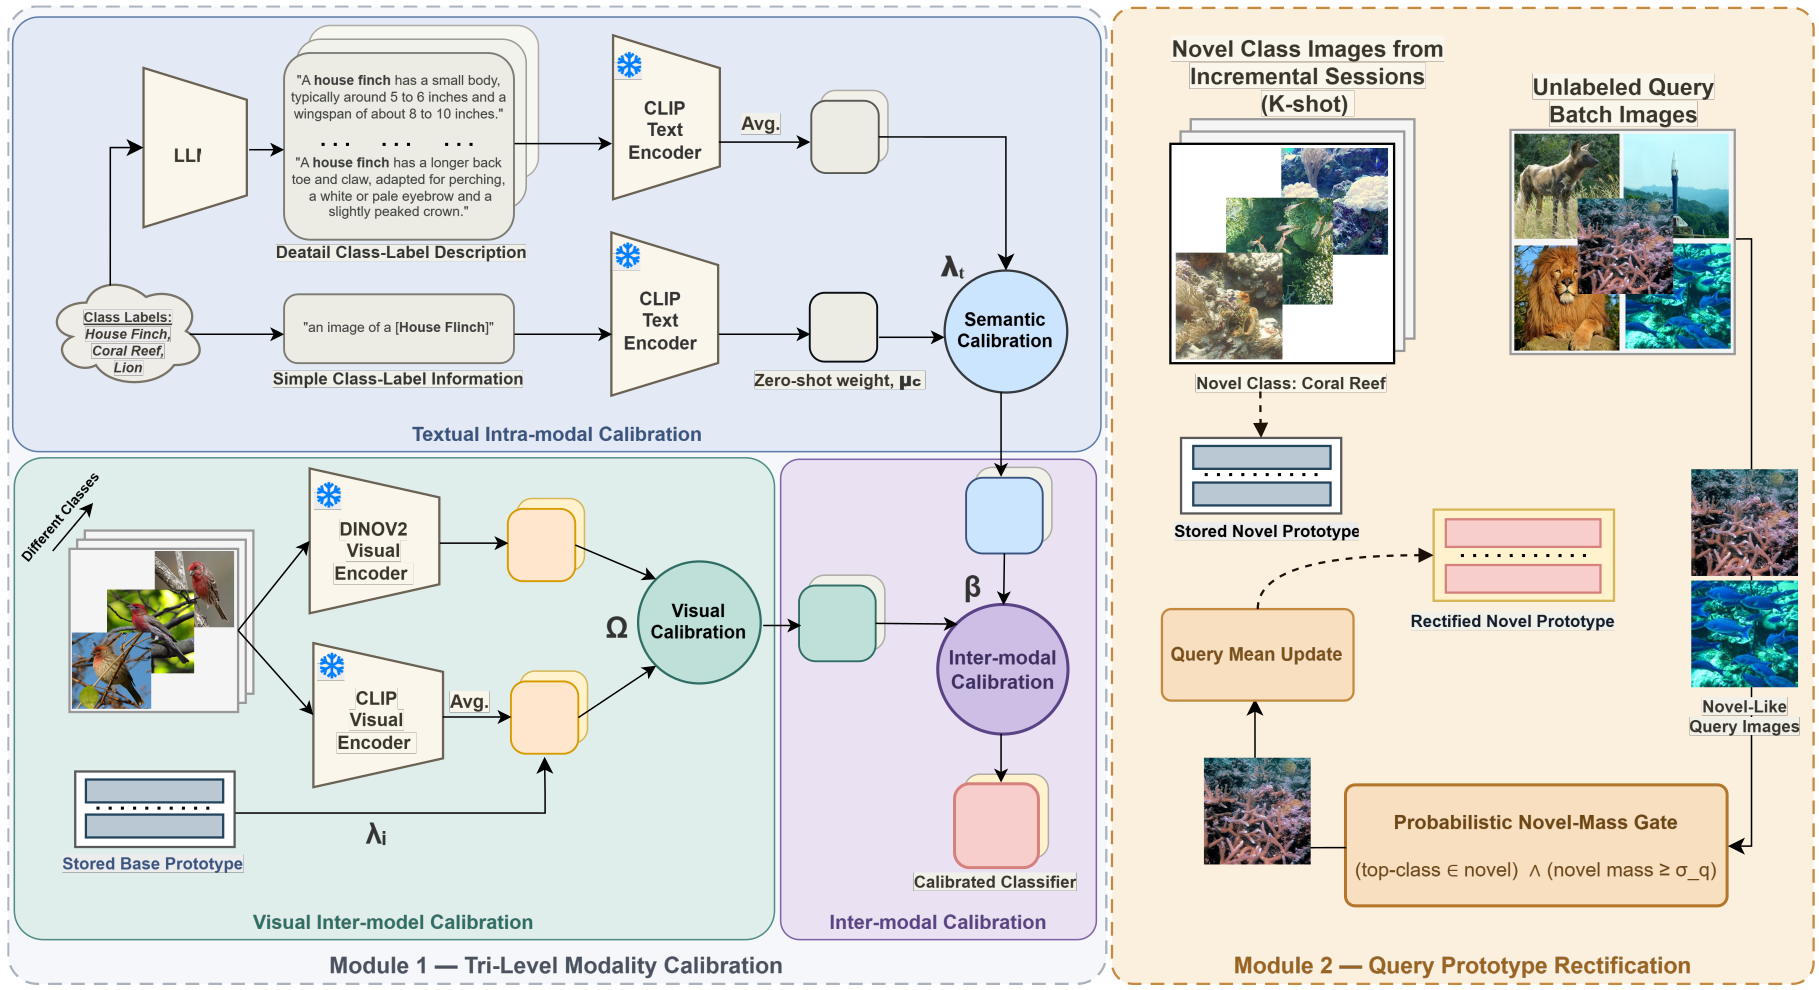
\includegraphics[width=\textwidth]{fig1_architecture}
    \caption{Overview of the two-module training-free FSCIL backbone studied in this thesis. Module~1 performs tri-level modality calibration (textual intra-modal, visual inter-model, and inter-modal calibration); Module~2 performs query prototype rectification, refining only novel DINOv2 prototypes through a precision-favoring gate. The Discriminative Prompt-based Recalibration module proposed in \autoref{sec:dpr} operates upstream of Module~1's textual intra-modal calibration and is not shown here, since it introduces no new images or query-side evidence, only an additional label-only refinement of the semantic prototype pipeline already depicted.}
    \label{fig:architecture}
\end{figure}

\section{Multi-Modal Prototypes}
\label{sec:prototypes}

\textbf{Encoder notation.} Let $f_I$ and $f_T$ be the frozen CLIP image and text encoders, and let $f_D$ be the frozen DINOv2 image encoder. For any nonzero vector $\mathbf{u}$, $\mathrm{norm}(\mathbf{u})$ denotes $\ell_2$ normalization. We use unit-normalized query and support features throughout: for any image $\mathbf{x}$,
\begin{equation}
    \mathrm{norm}(\mathbf{u}) = \frac{\mathbf{u}}{\lVert \mathbf{u} \rVert_2}, \qquad
    q_C(\mathbf{x}) = \mathrm{norm}\big(f_I(\mathbf{x})\big), \qquad
    q_D(\mathbf{x}) = \mathrm{norm}\big(f_D(\mathbf{x})\big).
    \label{eq:qnorm}
\end{equation}

\textbf{Semantic inputs.} For each class $c \in \mathcal{C}_{\le t}$, we use a class prompt $\pi_c$ (e.g., ``an image of a [class name]'') and $n_c$ description sentences $\{d_{c,r}\}_{r=1}^{n_c}$, drawn from a fixed prompt template and a pool of short, factual descriptions of the class (optionally produced once, offline, by an LLM). The prompt embedding $w_c$, each description embedding $z_{c,r}$, and the normalized description mean $\bar z_c$ are
\begin{equation}
    w_c = \mathrm{norm}\big(f_T(\pi_c)\big), \qquad
    z_{c,r} = \mathrm{norm}\big(f_T(d_{c,r})\big), \qquad
    \bar z_c = \mathrm{norm}\!\left(\frac{1}{n_c}\sum_{r=1}^{n_c} z_{c,r}\right).
    \label{eq:semanticinputs}
\end{equation}

\textbf{Visual prototypes.} For each observed class we build one CLIP visual prototype and one DINOv2 visual prototype from the same support set $\mathcal{X}_c$:
\begin{equation}
    v_{C,c} = \mathrm{norm}\!\left(\frac{1}{m_c}\sum_{j=1}^{m_c} q_C(\mathbf{x}_{c,j})\right), \qquad
    v_{D,c} = \mathrm{norm}\!\left(\frac{1}{m_c}\sum_{j=1}^{m_c} q_D(\mathbf{x}_{c,j})\right), \qquad c \in \mathcal{C}_{\le t}.
    \label{eq:visualprototypes}
\end{equation}
All four quantities---$w_c$, $\bar z_c$, $v_{C,c}$, $v_{D,c}$---are computed once per class and cached; no gradient ever flows through $f_I$, $f_T$, or $f_D$.

\section{Tri-Level Calibration (\textsc{TRiC})}
\label{sec:tric}

\textsc{TRiC} assembles the final classifier in three explicit levels, each responsible for calibrating one specific source of incompatibility.

\subsection{Level 1: Semantic Calibration}

A class prompt embedding $w_c$ is cheap to obtain but generic; a description mean $\bar z_c$ is more specific but is only as reliable as the description pool. Level~1 combines the two, before any visual evidence is used, with a single interpolation coefficient $\lambda_T \in [0,1]$ that controls how much description information enters the final semantic prototype $s_c$:
\begin{equation}
    s_c = \mathrm{norm}\big((1-\lambda_T)\, w_c + \lambda_T\, \bar z_c\big), \qquad 0 \le \lambda_T \le 1.
    \label{eq:level1}
\end{equation}
For a query image $\mathbf{x}$, the semantic score of class $c$ is the cosine similarity between the CLIP image embedding and the semantic prototype, which is well defined precisely because CLIP's joint image-text training aligns both in one space:
\begin{equation}
    \ell^S_c(\mathbf{x}) = q_C(\mathbf{x})^\top s_c, \qquad c \in \mathcal{C}_{\le t}.
    \label{eq:semanticscore}
\end{equation}

\subsection{Level 2: Inter-Model Visual Calibration}

The CLIP-image and DINOv2 branches first produce \emph{separate class-score vectors}---vectors of cosine similarities indexed by class---and are fused along this common axis rather than averaged in either encoder's raw embedding space. This is the key structural change relative to a bi-level (single-encoder) design: because $\ell^C_c(\mathbf{x})$ and $\ell^D_c(\mathbf{x})$ are both bounded cosine similarities in $[-1,1]$, they are already on a comparable scale and can be fused directly, with no per-branch rescaling required beforehand.
\begin{equation}
    \ell^C_c(\mathbf{x}) = q_C(\mathbf{x})^\top v_{C,c}, \qquad
    \ell^D_c(\mathbf{x}) = q_D(\mathbf{x})^\top v_{D,c}, \qquad
    \ell^V_c(\mathbf{x}) = \omega\, \ell^D_c(\mathbf{x}) + (1-\omega)\, \ell^C_c(\mathbf{x}), \qquad 0 \le \omega \le 1,
    \label{eq:level2}
\end{equation}
where $\ell^V_c(\mathbf{x})$ is the fused visual logit and the coefficient $\omega$ weights DINOv2 evidence against CLIP visual evidence.

\subsection{Level 3: Inter-Modal Calibration}

Semantic and visual evidence are fused at the logit level, and the result is converted into a proper posterior over $\mathcal{C}_{\le t}$ with a positive softmax scale $\rho$:
\begin{equation}
    \ell^F_c(\mathbf{x}) = \beta\, \ell^S_c(\mathbf{x}) + (1-\beta)\, \ell^V_c(\mathbf{x}), \qquad
    p_{\textsc{TRiC}}(c \mid \mathbf{x}) = \frac{\exp\big(\rho\, \ell^F_c(\mathbf{x})\big)}{\sum_{k \in \mathcal{C}_{\le t}} \exp\big(\rho\, \ell^F_k(\mathbf{x})\big)}, \qquad 0 \le \beta \le 1,\ \rho > 0,
    \label{eq:level3}
\end{equation}
where $\beta$ weights semantic evidence against visual evidence in the final decision. The classifier used to report accuracy at every session is $\hat y(\mathbf{x}) = \arg\max_{c} p_{\textsc{TRiC}}(c \mid \mathbf{x})$.

Because Level~2 is entirely visual and Level~3 is entirely a function of already-computed class scores, introducing DINOv2 costs one additional interpolation coefficient ($\omega$) rather than a full redesign of the fusion rule, and the semantic branch (Level~1) is left completely untouched by the presence of a second visual encoder---which is exactly the property that makes it possible to insert DPR (\autoref{sec:dpr}) upstream of Level~1 without altering Levels~2 or~3 at all.

\section{Query Prototype Rectification (QPR)}
\label{sec:qpr}

After Level~3 produces the calibrated posterior $p^*(c \mid \mathbf{x}) := p_{\textsc{TRiC}}(c \mid \mathbf{x})$, every novel-class DINOv2 prototype $v_{D,c}$, $c \in \mathcal{C}_n$, is still estimated from only $K$ images. The unlabeled query batch $\mathcal{U}_t$ contains additional structure, but it also contains base-class queries and, whenever the classifier is wrong, misclassified novel-class queries. QPR therefore uses $p^*$ only to \emph{select} a high-precision subset of $\mathcal{U}_t$ and updates only novel DINOv2 prototypes, leaving semantic prototypes, CLIP visual prototypes, and base DINOv2 prototypes entirely untouched.

\textbf{Gate.} For each query $\mathbf{x} \in \mathcal{U}_t$, define its overall prediction $\hat y(\mathbf{x})$, its best novel-class prediction $\hat y_n(\mathbf{x})$, and its total novel posterior mass $m_n(\mathbf{x})$:
\begin{equation}
    \hat y(\mathbf{x}) = \arg\max_{k \in \mathcal{C}_{\le t}} p^*(k \mid \mathbf{x}), \qquad
    \hat y_n(\mathbf{x}) = \arg\max_{k \in \mathcal{C}_n} p^*(k \mid \mathbf{x}), \qquad
    m_n(\mathbf{x}) = \sum_{k \in \mathcal{C}_n} p^*(k \mid \mathbf{x}).
    \label{eq:gatequantities}
\end{equation}
A query is admitted into the global gate $\mathcal{G}$ only if its top-class prediction is already novel \emph{and} its total novel posterior mass exceeds an admission threshold $\tau_q \in [0,1]$; admitted queries are then routed to a class-specific pool $\mathcal{G}_c$:
\begin{equation}
    \mathcal{G} = \{\mathbf{x} \in \mathcal{U}_t : \hat y(\mathbf{x}) \in \mathcal{C}_n \ \text{and} \ m_n(\mathbf{x}) \ge \tau_q\}, \qquad
    \mathcal{G}_c = \{\mathbf{x} \in \mathcal{G} : \hat y_n(\mathbf{x}) = c\}, \quad c \in \mathcal{C}_n.
    \label{eq:gate}
\end{equation}
If $|\mathcal{G}_c| < m_{\min}$ for a minimum pool size $m_{\min} \in \mathbb{N}$, class $c$ is judged not to have enough high-confidence evidence, and its prototype is left unchanged at $v_{D,c}$.

\textbf{Update.} For a novel class with a sufficiently large admitted pool, a probability-weighted DINOv2 query mean is computed, using each admitted query's own novel-class posterior as its weight:
\begin{equation}
    a_c(\mathbf{x}) = \frac{p^*(c \mid \mathbf{x})}{\sum_{\mathbf{x}' \in \mathcal{G}_c} p^*(c \mid \mathbf{x}')}, \qquad
    \tilde v_{D,c} = \mathrm{norm}\!\left(\sum_{\mathbf{x} \in \mathcal{G}_c} a_c(\mathbf{x})\, q_D(\mathbf{x})\right), \qquad \sum_{\mathbf{x} \in \mathcal{G}_c} a_c(\mathbf{x}) = 1.
    \label{eq:querymean}
\end{equation}
The rectified DINOv2 prototype is a convex interpolation between the original $K$-shot support prototype and the query mean, controlled by $\alpha \in [0,1]$; every other prototype is left unchanged:
\begin{equation}
    v'_{D,c} =
    \begin{cases}
        \mathrm{norm}\big((1-\alpha)\, v_{D,c} + \alpha\, \tilde v_{D,c}\big), & c \in \mathcal{C}_n \ \text{and} \ |\mathcal{G}_c| \ge m_{\min}, \\
        v_{D,c}, & \text{otherwise.}
    \end{cases}
    \label{eq:qprupdate}
\end{equation}
The rectified classifier is obtained by substituting $v'_{D,c}$ for $v_{D,c}$ in \autoref{eq:level2} and recomputing \autoref{eq:level3}. Every encoder and every other prototype remains frozen; QPR only ever touches the small subset of novel DINOv2 prototypes that both attract enough high-confidence queries and are themselves the object of a confident novel-class prediction.

\section{Discriminative Prompt-Based Recalibration (DPR)}
\label{sec:dpr}

QPR repairs residual novel-visual-prototype noise using unlabeled query evidence. It does nothing for the \emph{semantic} branch, and it does nothing at all for base classes, which never pass through its gate. This section presents Discriminative Prompt-based Recalibration (DPR), the methodological contribution proposed in this thesis: a label-only refinement of the Level-1 semantic prototypes $\{s_c\}_{c \in \mathcal{C}_{\le t}}$ that requires no images, novel or otherwise, and that is designed to reduce semantic confusion between pairs of classes whose prototypes are already highly similar before any visual evidence is considered at all.

\subsection{Motivation}

Level~1 (\autoref{eq:level1}) builds each class's semantic prototype independently of every other class. This is efficient, but it means that nothing in the \textsc{TRiC} pipeline as presented in \autoref{sec:tric} ever checks whether two classes' semantic prototypes are actually distinguishable from one another. On a coarse-grained benchmark this rarely matters, because most class pairs are already semantically distant. On a fine-grained benchmark, however, many class pairs are close relatives by construction (e.g., two tern species, or two warbler species), and it is entirely possible for their semantic prototypes to end up so similar that the semantic branch of \autoref{eq:level3} cannot meaningfully separate them, forcing the classifier to rely on the visual branch alone in exactly the cases where the visual evidence is itself scarce (novel classes) or ambiguous. \autoref{sec:casestudy} presents a concrete, documented instance of this failure mode on CUB-200. DPR is designed to reduce it directly, by identifying confusable class pairs after prototypes are built, and sharpening their separation using prompts explicitly written to be contrastive between that specific pair.

\subsection{Pairwise Discriminative Prompting}

Let $T_c \equiv s_c$ denote the Level-1 semantic prototype of class $c$ (we keep the symbol $T_c$ in this section to make the recalibration equations self-contained). Because every $T_c$ is unit-normalized, the pairwise semantic similarity between classes $i$ and $j$ is simply their cosine similarity,
\begin{equation}
    S_{i,j} = T_i^\top T_j, \qquad i \ne j, \qquad S_{i,j} = S_{j,i}.
    \label{eq:dprsim}
\end{equation}
For every ordered pair of classes $(i,j)$ with $i \ne j$, we assume a fixed pool of $K_p$ \emph{discriminative prompts} $\{\pi_{i,j,1}, \dots, \pi_{i,j,K_p}\}$ (we use $K_p = 3$ throughout), each written so as to describe class $i$ in a way that explicitly contrasts it with class $j$ (for example, a template of the form ``Unlike a \{class $j$\}, a \{class $i$\} typically has \dots''). These prompts can be generated once, offline, by an LLM or by a domain expert, exactly as the description pool $\{d_{c,r}\}$ already used in \autoref{eq:semanticinputs} is generated; generating them requires only the list of class names, not a single training image. Passing all $K_p$ prompts of the pair $(i,j)$ through the frozen CLIP text encoder and averaging gives the pairwise discriminative prototype of class $i$ relative to class $j$:
\begin{equation}
    N_{i,j} = \mathrm{norm}\!\left(\frac{1}{K_p}\sum_{k=1}^{K_p} f_T(\pi_{i,j,k})\right).
    \label{eq:discprototype}
\end{equation}
For $n = |\mathcal{C}_{\le t}|$ classes there are $n(n-1)$ such directed discriminative prototypes; because \autoref{eq:discprototype} depends only on class names and prompts, all of them can be pre-computed once, offline, in parallel, with no dependency on any support or query image.

\subsection{Iterative Recalibration Algorithm}

DPR proceeds in rounds. At each round it identifies the single most confusable, not-yet-visited pair of classes, attempts to recalibrate both of their semantic prototypes away from each other using \autoref{eq:discprototype}, and accepts each side of the recalibration independently, subject to a safeguard that rejects any update which would make the affected class more confusable with the rest of the class set than a small tolerance allows.

\textbf{Selection.} Maintain a set $\mathcal{V}$ of already-visited unordered class pairs, initially empty. At each round, let
\begin{equation}
    (a,b) = \arg\max_{\{i,j\} \notin \mathcal{V}} S_{i,j}.
    \label{eq:dprselect}
\end{equation}
If $S_{a,b}$ does not exceed a fixed threshold $\theta$ (we use $\theta = 0.5$, following the same threshold used in the original design of this mechanism), or if every pair has already been visited, the algorithm terminates: no remaining pair is confusable enough to justify recalibration.

\textbf{Proposed update.} Ties in \autoref{eq:dprselect} are broken arbitrarily. Mark $\{a,b\}$ as visited. Build a discrimination-weighted pull vector for each side of the pair, aggregating the discriminative prototypes of $a$ (respectively $b$) relative to every \emph{other} class, weighted by how similar $a$ (respectively $b$) already is to that class:
\begin{equation}
    D_{a \to b} = \sum_{i \ne a} S_{a,i}\, N_{a,i}, \qquad
    D_{b \to a} = \sum_{i \ne b} S_{b,i}\, N_{b,i}.
    \label{eq:dprpull}
\end{equation}
Intuitively, $D_{a \to b}$ reuses the discriminative evidence already computed for every other class in the dataset to pull $T_a$ toward a description of class $a$ that is simultaneously informed by how class $a$ relates to the rest of the class set, not only to $b$. A candidate pair of recalibrated prototypes is then formed with a step size $\gamma \in [0,1]$:
\begin{equation}
    T'_a = \mathrm{norm}\big(T_a + \gamma\, D_{a \to b}\big), \qquad
    T'_b = \mathrm{norm}\big(T_b + \gamma\, D_{b \to a}\big).
    \label{eq:dprcandidate}
\end{equation}

\textbf{Acceptance test.} The candidate prototypes are not accepted unconditionally. First, recompute the similarity of the two candidates to every class, including each other:
\begin{equation}
    \mathrm{tmp}_{a',b'} = T_a'^\top T_b', \qquad
    \mathrm{tmp}_{a',i} = T_a'^\top T_i,\quad
    \mathrm{tmp}_{b',i} = T_b'^\top T_i, \qquad i \ne a, b.
    \label{eq:dprtmp}
\end{equation}
The recalibration is judged worth considering at all only if it actually reduced the confusion between $a$ and $b$:
\begin{equation}
    S_{a,b} > \mathrm{tmp}_{a',b'}.
    \label{eq:dprtest1}
\end{equation}
If \autoref{eq:dprtest1} holds, each side is then \emph{independently} tested against collateral damage to its separation from every other class, using a fixed margin $\epsilon$ (we use $\epsilon = 0.1$):
\begin{equation}
    \sum_{\substack{i \ne a \\ i \ne b}} S_{a,i} \ - \sum_{\substack{i \ne a \\ i \ne b}} \mathrm{tmp}_{a',i} \ > \ -\epsilon
    \quad \Longrightarrow \quad T_a \leftarrow T'_a,
    \label{eq:dprtest2a}
\end{equation}
\begin{equation}
    \sum_{\substack{i \ne a \\ i \ne b}} S_{b,i} \ - \sum_{\substack{i \ne a \\ i \ne b}} \mathrm{tmp}_{b',i} \ > \ -\epsilon
    \quad \Longrightarrow \quad T_b \leftarrow T'_b .
    \label{eq:dprtest2b}
\end{equation}
\autoref{eq:dprtest2a} and \autoref{eq:dprtest2b} read: the new \emph{aggregate} similarity of the recalibrated class to every remaining class must not exceed its old aggregate similarity by more than $\epsilon$. Each side is accepted or rejected on its own; it is possible for only $T_a$, only $T_b$, both, or neither to be updated in a given round. Whenever a prototype is updated, its row of the similarity matrix $S$ is refreshed from the corresponding $\mathrm{tmp}$ values before the next round begins. The algorithm then returns to the selection step and repeats until termination.

\autoref{alg:dpr} gives the complete procedure.

\begin{algorithm}[H]
\caption{Discriminative Prompt-based Recalibration (DPR)}
\label{alg:dpr}
\begin{algorithmic}[1]
\Require semantic prototypes $\{T_c\}_{c \in \mathcal{C}_{\le t}}$, discriminative prototypes $\{N_{i,j}\}$, threshold $\theta$, margin $\epsilon$, step size $\gamma$
\Ensure recalibrated semantic prototypes $\{T_c\}_{c \in \mathcal{C}_{\le t}}$
\State $\mathcal{V} \gets \emptyset$
\State $S_{i,j} \gets T_i^\top T_j$ for all $i \ne j$
\Loop
    \State $(a,b) \gets \arg\max_{\{i,j\} \notin \mathcal{V}} S_{i,j}$
    \If{no such pair remains, or $S_{a,b} \le \theta$}
        \State \textbf{break}
    \EndIf
    \State $\mathcal{V} \gets \mathcal{V} \cup \{\{a,b\}\}$
    \State $D_{a \to b} \gets \sum_{i \ne a} S_{a,i}\, N_{a,i}$; \quad $D_{b \to a} \gets \sum_{i \ne b} S_{b,i}\, N_{b,i}$
    \State $T'_a \gets \mathrm{norm}(T_a + \gamma D_{a \to b})$; \quad $T'_b \gets \mathrm{norm}(T_b + \gamma D_{b \to a})$
    \State recompute $\mathrm{tmp}_{a',b'}$, $\mathrm{tmp}_{a',i}$, $\mathrm{tmp}_{b',i}$ for all $i \ne a,b$
    \If{$S_{a,b} > \mathrm{tmp}_{a',b'}$}
        \If{$\sum_{i \ne a,b} S_{a,i} - \sum_{i \ne a,b} \mathrm{tmp}_{a',i} > -\epsilon$}
            \State $T_a \gets T'_a$; refresh $S_{a,i} \gets \mathrm{tmp}_{a',i}$ for all $i \ne a$
        \EndIf
        \If{$\sum_{i \ne a,b} S_{b,i} - \sum_{i \ne a,b} \mathrm{tmp}_{b',i} > -\epsilon$}
            \State $T_b \gets T'_b$; refresh $S_{b,i} \gets \mathrm{tmp}_{b',i}$ for all $i \ne b$
        \EndIf
    \EndIf
\EndLoop
\State \Return $\{T_c\}_{c \in \mathcal{C}_{\le t}}$
\end{algorithmic}
\end{algorithm}

\subsection{Termination and Complexity}

Every iteration of the loop in \autoref{alg:dpr} adds exactly one previously unvisited pair to $\mathcal{V}$, and there are only $\binom{n}{2}$ unordered pairs among $n = |\mathcal{C}_{\le t}|$ classes, so the loop terminates after at most $\binom{n}{2}$ rounds even if the threshold check never triggers first. Each round performs $O(n)$ work to build $D_{a \to b}$ and $D_{b \to a}$ and $O(n)$ work to recompute the affected similarity row, so the total cost of \autoref{alg:dpr} is $O(n^3)$ in the worst case, plus a one-time $O(n^2 K_p)$ cost to compute every discriminative prototype $N_{i,j}$, which is embarrassingly parallel and can be cached offline since it does not depend on any support or query image. For the class counts used in this thesis's experimental setting ($n \le 200$; \autoref{chapter:experiments}), this cost is negligible relative to a single forward pass of the CLIP or DINOv2 visual encoders over a session's images.

\subsection{Worked Illustrative Example}
\label{sec:dprexample}

The following walkthrough uses hypothetical, illustrative similarity values chosen only to demonstrate the mechanics of \autoref{alg:dpr}; they are not measured quantities. Consider four classes among the incremental classes of a fine-grained bird benchmark: two visually similar tern species, Caspian Tern ($a$) and Elegant Tern ($b$), and two better-separated classes, Least Tern ($d$) and a base-session sparrow class ($e$) --- deliberately chosen to echo the real confusion pattern documented in \autoref{sec:casestudy}. Suppose the baseline pairwise semantic similarities are
\[
S_{a,b} = 0.62, \quad S_{a,d} = 0.31, \quad S_{a,e} = 0.18, \quad S_{b,d} = 0.27, \quad S_{b,e} = 0.22, \quad S_{d,e} = 0.35 .
\]
Since $S_{a,b} = 0.62$ is both the largest pairwise similarity and exceeds $\theta = 0.5$, the pair $(a,b)$ is selected first (\autoref{eq:dprselect}). \autoref{eq:dprpull} combines the discriminative prompts contrasting $a$ from $b$ (and $b$ from $a$) with the existing similarity of each class to every other class, and \autoref{eq:dprcandidate} forms the candidate prototypes with step size $\gamma = 0.5$. Suppose the resulting candidates satisfy $\mathrm{tmp}_{a',b'} = 0.41$, so that \autoref{eq:dprtest1} holds ($0.62 > 0.41$): the pairwise confusion between Caspian Tern and Elegant Tern has indeed been reduced, and both sides proceed to the margin test. Suppose further that class $a$'s aggregate similarity to the remaining classes $\{d,e\}$ moves from $S_{a,d} + S_{a,e} = 0.49$ to $\mathrm{tmp}_{a',d} + \mathrm{tmp}_{a',e} = 0.53$, a change of $-0.04$, which satisfies \autoref{eq:dprtest2a} ($-0.04 > -0.1$), so $T_a$ is updated. Suppose, on the other hand, that class $b$'s aggregate similarity to $\{d,e\}$ moves from $0.49$ to $0.61$, a change of $-0.12$, which \emph{fails} \autoref{eq:dprtest2b} ($-0.12 \not> -0.1$): sharpening Elegant Tern away from Caspian Tern would, in this hypothetical instance, have pushed it close enough to Least Tern and the sparrow class to cost more than it gained, so $T_b$ is left unchanged. The net outcome of this round is therefore asymmetric --- exactly the kind of per-side, per-class conservatism that \autoref{eq:dprtest2a}--\autoref{eq:dprtest2b} are designed to produce --- after which the algorithm returns to \autoref{eq:dprselect} and looks for the next most confusable remaining pair.

\subsection{Discussion of Design Choices}

The acceptance test in \autoref{eq:dprtest2a}--\autoref{eq:dprtest2b} compares \emph{aggregate} similarity to the remaining classes before and after recalibration, rather than the similarity to the single closest remaining class. The aggregate form is simpler to compute and to reason about (it only requires two scalar sums per side per round), but it can in principle accept an update that trades a small aggregate improvement for a large increase in confusion with one specific third class. A per-class (maximum-based) variant of \autoref{eq:dprtest2a}--\autoref{eq:dprtest2b}, which would instead require that similarity to \emph{every} individual remaining class increase by no more than $\epsilon$, is a strictly stricter and, we believe, promising alternative that we leave to future empirical comparison (\autoref{sec:futurework}). Likewise, the step size $\gamma$ is left as an open hyperparameter in the original design of this mechanism; we propose $\gamma = 0.5$ as a reasonable default, by analogy with QPR's default interpolation weight, but its empirical validation is future work. Finally, DPR is deliberately restricted to touching only the semantic prototypes $T_c$: it never reads a support or query image, which keeps it exactly as label-efficient as the class-description pool already used by Level~1, and keeps it entirely decoupled from, and safely composable with, QPR's separate query-side visual rectification.

\section{Integration and Overall Pipeline}
\label{sec:integration}

The three mechanisms presented in this chapter operate on three disjoint sources of evidence, in increasing order of what they require: DPR (\autoref{sec:dpr}) requires only class labels and prompts and can run entirely offline, before a single support or query image for a session has even been observed; the three levels of \textsc{TRiC} (\autoref{sec:tric}) require the $K$-shot labeled support set of each new class; and QPR (\autoref{sec:qpr}) requires the unlabeled query batch that only becomes available once a session is underway. This ordering is also a supervision-strength ordering, from least to most session-specific evidence, and the pipeline is applied in exactly this order: DPR recalibrates the semantic prototypes $\{T_c\}$ once, offline; \textsc{TRiC} then builds and fuses semantic and visual evidence (\autoref{eq:level1}--\autoref{eq:level3}) using the DPR-recalibrated $T_c$ in place of the raw Level-1 output $s_c$, with everything else in \autoref{sec:tric} unchanged; and QPR (\autoref{eq:gatequantities}--\autoref{eq:qprupdate}) then consumes the resulting calibrated posterior $p^*(c\mid\mathbf{x})$ as its gate signal, exactly as it would without DPR. Because DPR only ever replaces the input to \autoref{eq:semanticscore} and touches no other equation, and because QPR only ever reads $p^*(c\mid\mathbf{x})$ and writes to $v_{D,c}$, all three mechanisms compose without any structural conflict: every encoder, and every prototype not explicitly targeted by DPR or QPR, remains exactly as frozen as in the original two-module design of \autoref{fig:architecture}.


\chapter{Experimental Setup}
\label{chapter:experiments}

This chapter describes the datasets, protocol, baselines, and implementation details used to evaluate the validated part of the pipeline, \textsc{TRiC} and \textsc{TRiC}-QPR (\autoref{chapter:results}), and the protocol we propose for the future empirical validation of DPR.

\section{Datasets and Protocol}

We use the three standard FSCIL benchmarks and their standard protocols \autocite{tao2020fewshot, chen2025bimc}, summarized in \autoref{tab:datasets}.

\begin{table}[H]
    \centering
    \begin{tabular}{l c c c c c}
        \toprule
        Dataset & Base classes & Incremental sessions & Way & Shot & Total classes \\
        \midrule
        CIFAR-100 \autocite{krizhevsky2009learning} & 60 & 8 & 5 & 5 & 100 \\
        \emph{mini}ImageNet \autocite{vinyals2016matching} & 60 & 8 & 5 & 5 & 100 \\
        CUB-200 \autocite{wah2011caltech} & 100 & 10 & 10 & 5 & 200 \\
        \bottomrule
    \end{tabular}
    \caption{FSCIL benchmarks used in this thesis. ``Way'' is the number of new classes introduced per incremental session and ``shot'' is the number of labeled images per new class.}
    \label{tab:datasets}
\end{table}

CIFAR-100 and \emph{mini}ImageNet use 60 base classes and eight 5-way 5-shot incremental sessions (sessions $A_0$ through $A_8$); CUB-200-2011, a fine-grained bird recognition dataset, uses 100 base classes and ten 10-way 5-shot incremental sessions (sessions $A_0$ through $A_{10}$), and is the benchmark on which fine-grained inter-class confusability (\autoref{sec:dpr}) is most pronounced. Following standard practice, we report accuracy at every session, averaged over 20 random seeds per configuration, with a fixed, non-overlapping evaluation query set drawn from every class observed so far.

\section{Implementation Details}

All variants use a frozen CLIP ViT-B/16 image and text encoder \autocite{radford2021learning}; \textsc{TRiC} additionally uses a frozen DINOv2 ViT-L/14 image encoder \autocite{oquab2023dinov2}, which is comparable in computational cost (FLOPs) to the CLIP image encoder, so the dominant inference cost of \textsc{TRiC}-QPR is approximately twice that of a CLIP-only frozen FSCIL method. Class descriptions and prompt templates follow \textcite{chen2025bimc}. Unless otherwise noted, we use the deployed default hyperparameters: $\lambda_T = 0.5$; inter-model weight $\omega = 0.7$; softmax scale $\rho = 100$; inter-modal weight $\beta = 0.65$ on CIFAR-100 and \emph{mini}ImageNet and $\beta = 0.30$ on CUB-200 (the only hyperparameter allowed to vary by dataset, following the convention of the predecessor framework \autocite{chen2025bimc}); and QPR defaults $\tau_q = 0.3$, $m_{\min} = 5$, $\alpha = 0.75$, fixed across all three datasets and all seeds, i.e., with no per-seed tuning.

\section{Baselines}

We compare against zero-shot and training-free baselines spanning the language-only, visual-only, and vision-language design points discussed in \autoref{chapter:related}: \textbf{CLIP zero-shot}, which classifies directly with CLIP's prompt embedding and no visual prototype at all; \textbf{Visual Prototype (CLIP)}, a plain CLIP nearest-visual-prototype classifier with no calibration; \textbf{TEEN} \autocite{wang2023teen}; \textbf{FeCAM} \autocite{goswami2023fecam}; \textbf{BiMC} and \textbf{BiMC (ensemble)} \autocite{chen2025bimc}, the latter including BiMC's full base-covariance and description-nearest-neighbor auxiliary branches; and two single-encoder ablations of the framework studied in this thesis, \textbf{CLIP-visual-only} and \textbf{DINO-visual-only}, each restricting Level~2 (\autoref{eq:level2}) to a single visual encoder.

\section{Evaluation Metrics}

We report four complementary metrics throughout \autoref{chapter:results}: (i) session-wise accuracy $A_t$, the fraction of the cumulative test set (every class observed up to and including session $t$) correctly classified at session $t$; (ii) average accuracy, the mean of $A_0, \dots, A_T$ across all sessions; (iii) performance degradation, $\mathrm{PD} = A_0 - A_T$, the drop from base-session to final-session accuracy, which isolates how much of a method's base-session advantage survives the incremental stream; and (iv) a final-session Full/Base/Novel decomposition, which separately reports accuracy on the base classes $\mathcal{C}_b$, the novel classes $\mathcal{C}_n$, and their union, at the final session $T$. For QPR specifically, we additionally report gate purity (the fraction of gated queries whose true class is indeed novel), base leakage (its complement), the number of gated queries, and the number of novel classes whose prototype was actually updated (\autoref{sec:qprresults}).

\section{Proposed Protocol for DPR}

Because DPR (\autoref{sec:dpr}) has not yet been evaluated empirically, we specify here the protocol under which we propose it should be validated, so that the qualitative and quantitative discussion in \autoref{sec:dprresults} can be read as a concrete, falsifiable plan rather than a vague direction. We propose: (i) generating the discriminative prompt pool $\{\pi_{i,j,k}\}$ once per dataset, offline, using the same LLM and prompting infrastructure already used for the description pool $\{d_{c,r}\}$; (ii) running \autoref{alg:dpr} once per session, immediately after Level~1 and before Level~2, on the accumulated class set $\mathcal{C}_{\le t}$; (iii) reporting the same session-wise, Full/Base/Novel, and PD metrics defined above, with and without DPR, on top of an otherwise identical \textsc{TRiC}-QPR pipeline; and (iv) reporting an \emph{intra-novel contamination rate}---the fraction of admitted-novel queries (\autoref{eq:gate}) whose predicted novel class differs from their true novel class---both with and without DPR, since this is the specific failure mode DPR targets and it is not visible in gate purity alone (\autoref{sec:casestudy}).


\chapter{Results and Discussion}
\label{chapter:results}

This chapter presents the empirical results of \textsc{TRiC} and \textsc{TRiC}-QPR, drawn from the evaluation protocol of \autoref{chapter:experiments}, followed by a design-validation discussion of the proposed DPR module.

\section{Main Results}
\label{sec:mainresults}

\autoref{fig:sessionacc} plots session-wise accuracy for every method on all three datasets. Across all three benchmarks, \textsc{TRiC} and \textsc{TRiC}-QPR dominate every baseline throughout the incremental schedule, not only at the final session, and the gap between them and the strongest prior training-free baseline (BiMC with its full auxiliary ensemble) widens rather than narrows as more novel classes accumulate. Without any incremental training, the tri-level backbone improves on the BiMC ensemble baseline's final-session accuracy by $+9.83$, $+1.32$, and $+12.53$ points on CIFAR-100, \emph{mini}ImageNet, and CUB-200 respectively ($73.24 \rightarrow 83.07$, $92.41 \rightarrow 93.73$, $72.76 \rightarrow 85.29$), and the label-free QPR stage adds a further $+2.43$, $+1.01$, and $+0.88$ points on top of the same backbone ($83.07\rightarrow 85.50$, $93.73\rightarrow94.74$, $85.29\rightarrow86.17$). \textsc{TRiC}-QPR beats BiMC in all 20 evaluated seeds on every benchmark, and, as \autoref{sec:qprresults} shows, these gains do not come at the price of base-class confusion.

\begin{figure}[H]
    \centering
    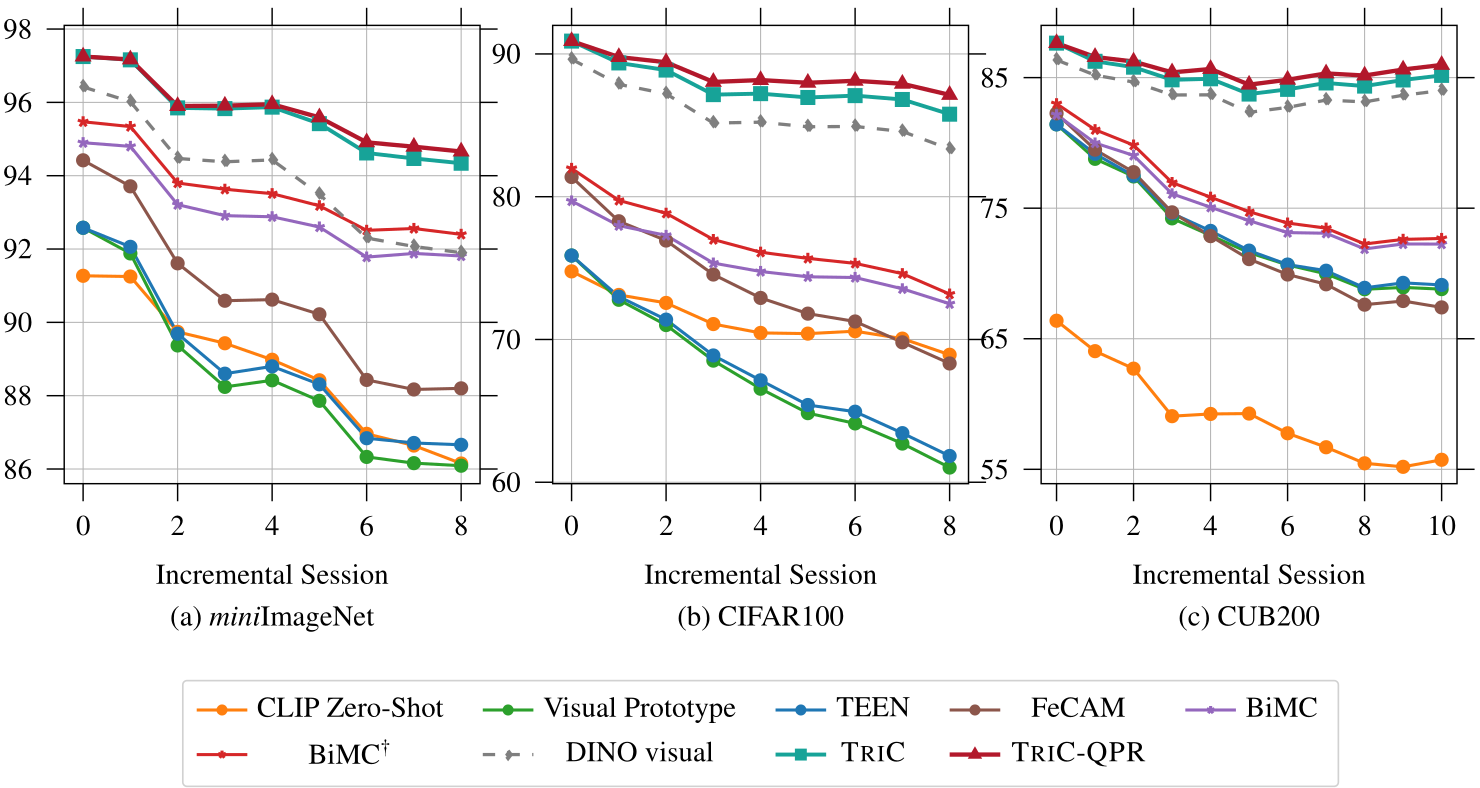
\includegraphics[width=\textwidth]{fig2_session_accuracy}
    \caption{Session-wise accuracy on (a) \emph{mini}ImageNet, (b) CIFAR-100, and (c) CUB-200. \textsc{TRiC} and \textsc{TRiC}-QPR dominate every training-free baseline throughout the incremental schedule, not only at the final session.}
    \label{fig:sessionacc}
\end{figure}

\autoref{tab:minisession} summarizes the \emph{mini}ImageNet comparison at the initial (base), final, and average session, alongside performance degradation; the fully detailed, session-by-session comparisons for CIFAR-100 and CUB-200 are given in \autoref{tab:cifarsession} and \autoref{tab:cubsession}.

\begin{table}[H]
    \centering
    \begin{tabular}{l c c c c c}
        \toprule
        Method & Modality & $A_0$ & $A_8$ (final) & Avg. $\uparrow$ & PD $\downarrow$ \\
        \midrule
        CLIP zero-shot & L & 91.27 & 86.15 & 88.76 & 5.12 \\
        Visual Prototype (CLIP) & V & 92.58 & 86.09 & 88.50 & 6.49 \\
        TEEN & V & 92.58 & 86.66 & 88.86 & 5.92 \\
        FeCAM & V & 94.42 & 88.20 & 90.73 & 6.22 \\
        BiMC & V-L & 94.90 & 91.81 & 93.01 & 3.09 \\
        BiMC (ensemble) & V-L & 95.47 & 92.40 & 93.56 & 3.07 \\
        CLIP-visual-only & V & 92.58 & 86.79 & 88.92 & 5.79 \\
        DINO-visual-only & V & 96.42 & 91.90 & 93.94 & 4.52 \\
        \textsc{TRiC} & V-L & 96.64 & 93.73 & 95.65 & 2.91 \\
        \textsc{TRiC}-QPR & V-L & 96.64 & \textbf{94.74} & $\approx$95.9 & \textbf{1.90} \\
        \bottomrule
    \end{tabular}
    \caption{Session-wise comparison on \emph{mini}ImageNet, condensed to the base session ($A_0$), final session ($A_8$), 9-session average, and performance degradation (PD $= A_0 - A_8$). V, L, and V-L denote visual, language, and vision-language modalities. The full nine-session trajectory is plotted in \autoref{fig:sessionacc}(a).}
    \label{tab:minisession}
\end{table}

\begin{table}[H]
    \centering
    \small
    \begin{tabular}{l c c c c c c c c c c c c}
        \toprule
        Method & Mod. & $A_0$ & $A_1$ & $A_2$ & $A_3$ & $A_4$ & $A_5$ & $A_6$ & $A_7$ & $A_8$ & Avg.$\uparrow$ & PD$\downarrow$ \\
        \midrule
        CLIP zero-shot & L & 74.77 & 73.12 & 72.56 & 71.08 & 70.46 & 70.41 & 70.58 & 70.06 & 68.93 & 71.33 & 5.84 \\
        Visual Prototype (CLIP) & V & 75.88 & 72.78 & 71.01 & 68.52 & 66.55 & 64.84 & 64.12 & 62.71 & 61.03 & 67.49 & 14.85 \\
        TEEN & V & 75.88 & 73.00 & 71.39 & 68.88 & 67.14 & 65.41 & 64.94 & 63.44 & 61.84 & 67.99 & 14.04 \\
        FeCAM & V & 81.38 & 78.28 & 76.93 & 74.55 & 72.91 & 71.81 & 71.26 & 69.80 & 68.32 & 73.92 & 13.06 \\
        BiMC & V-L & 79.70 & 77.97 & 77.29 & 75.35 & 74.76 & 74.39 & 74.34 & 73.55 & 72.50 & 75.54 & 7.20 \\
        BiMC (ens.) & V-L & 81.98 & 79.74 & 78.84 & 77.00 & 76.11 & 75.68 & 75.33 & 74.61 & 73.18 & 76.94 & 8.80 \\
        CLIP-visual-only & V & 75.90 & 72.74 & 70.97 & 68.31 & 66.54 & 65.49 & 64.94 & 63.73 & 62.20 & 67.87 & 13.70 \\
        DINO-visual-only & V & 89.63 & 87.87 & 87.21 & 85.16 & 85.22 & 84.90 & 84.92 & 84.57 & 83.34 & 85.87 & 6.29 \\
        \textsc{TRiC} & V-L & 90.90 & 89.37 & 88.87 & 87.15 & 87.22 & 86.95 & 87.08 & 86.81 & 85.78 & 87.79 & 5.12 \\
        \textsc{TRiC}-QPR & V-L & 90.90 & 89.78 & 89.42 & 88.04 & 88.17 & 87.98 & 88.12 & 87.91 & 87.13 & \textbf{88.61} & \textbf{3.77} \\
        \bottomrule
    \end{tabular}
    \caption{Full session-wise comparison on CIFAR-100 (nine sessions, $A_0$--$A_8$).}
    \label{tab:cifarsession}
\end{table}

\begin{table}[H]
    \centering
    \small
    \begin{tabular}{l c c c c c c c c c c c c c}
        \toprule
        Method & Mod. & $A_0$ & $A_1$ & $A_2$ & $A_3$ & $A_4$ & $A_5$ & $A_6$ & $A_7$ & $A_8$ & $A_9$ & $A_{10}$ & Avg.$\uparrow$/PD$\downarrow$ \\
        \midrule
        CLIP zero-shot & L & 66.38 & 64.05 & 62.71 & 59.07 & 59.24 & 59.27 & 57.76 & 56.69 & 55.46 & 55.19 & 55.73 & 59.23 / 10.65 \\
        Visual Prot. (CLIP) & V & 81.42 & 78.78 & 77.43 & 74.22 & 72.91 & 71.59 & 70.65 & 69.97 & 68.79 & 68.93 & 68.80 & 73.04 / 12.62 \\
        TEEN & V & 81.42 & 79.16 & 77.49 & 74.60 & 73.26 & 71.75 & 70.68 & 70.21 & 68.90 & 69.28 & 69.12 & 73.26 / 12.30 \\
        FeCAM & V & 82.26 & 79.48 & 77.76 & 74.68 & 72.86 & 71.10 & 69.92 & 69.17 & 67.61 & 67.89 & 67.40 & 72.74 / 14.86 \\
        BiMC & V-L & 82.16 & 79.99 & 79.04 & 76.10 & 75.07 & 74.04 & 73.13 & 73.08 & 71.88 & 72.26 & 72.25 & 75.36 / 9.91 \\
        BiMC (ens.) & V-L & 83.00 & 81.01 & 79.83 & 76.96 & 75.84 & 74.73 & 73.86 & 73.47 & 72.26 & 72.61 & 72.68 & 76.02 / 10.32 \\
        CLIP-visual-only & V & 81.63 & 79.14 & 77.49 & 74.24 & 73.26 & 71.68 & 70.81 & 70.03 & 68.53 & 68.72 & 68.47 & 73.09 / 13.16 \\
        DINO-visual-only & V & 86.35 & 85.19 & 84.66 & 83.67 & 83.68 & 82.34 & 82.72 & 83.28 & 83.14 & 83.65 & 84.01 & 83.88 / 2.34 \\
        \textsc{TRiC} & V-L & 87.64 & 86.25 & 85.80 & 84.83 & 84.91 & 83.74 & 84.10 & 84.59 & 84.35 & 84.82 & 85.17 & 85.12 / 2.47 \\
        \textsc{TRiC}-QPR & V-L & 87.64 & 86.58 & 86.23 & 85.40 & 85.66 & 84.46 & 84.84 & 85.32 & 85.16 & 85.62 & 85.97 & \textbf{85.72 / 1.67} \\
        \bottomrule
    \end{tabular}
    \caption{Full session-wise comparison on CUB-200-2011 (eleven sessions, $A_0$--$A_{10}$).}
    \label{tab:cubsession}
\end{table}

Two patterns are visible across \autoref{tab:minisession}--\autoref{tab:cubsession}. First, \textsc{TRiC}'s advantage over every training-free baseline is present from the base session onward and grows with the number of incremental sessions, confirming that the gain is structural (better calibration) rather than an artifact of a particular session count. Second, QPR's contribution is concentrated in performance degradation rather than in base-session accuracy: on every dataset, $A_0$ is identical for \textsc{TRiC} and \textsc{TRiC}-QPR (QPR has no novel classes to rectify before any incremental session has occurred), and the entire QPR gain accumulates from $A_1$ onward as novel classes are introduced.

\section{Component Ablation of \textsc{TRiC}}
\label{sec:ablation}

\autoref{tab:ablation} isolates the contribution of each of the three calibration levels on \emph{mini}ImageNet by enabling only valid subsets of the semantic (Sem.), CLIP-visual (C-Vis.), and DINOv2-visual (D-Vis.) branches.

\begin{table}[H]
    \centering
    \begin{tabular}{c c c c c}
        \toprule
        Sem. & C-Vis. & D-Vis. & Avg. accuracy $\uparrow$ & PD $\downarrow$ \\
        \midrule
        \checkmark & & & 91.05 & 3.96 \\
         & \checkmark & & 88.92 & 5.79 \\
        \checkmark & \checkmark & & 92.97 & 3.09 \\
         & \checkmark & \checkmark & 94.37 & 4.32 \\
        \checkmark & \checkmark & \checkmark & \textbf{95.65} & \textbf{2.91} \\
        \bottomrule
    \end{tabular}
    \caption{Component ablation of \textsc{TRiC} on \emph{mini}ImageNet. The third row (Sem.\ + C-Vis., with no DINOv2 evidence) is structurally equivalent to the BiMC baseline; the bottom row is the full \textsc{TRiC} backbone.}
    \label{tab:ablation}
\end{table}

Three contrasts carry the argument for a tri-level, rather than bi-level, design. First, DINOv2 alone (Avg.\ $93.94$, PD $4.52$) exceeds CLIP-visual alone (Avg.\ $88.92$, PD $5.79$) by $5.02$ average points, confirming that DINOv2 is the stronger low-shot visual carrier on this benchmark and is therefore worth introducing at all. Second, the semantic-plus-CLIP-visual row, which is structurally the same combination BiMC uses, reaches Avg.\ $92.97$---already \emph{below} DINOv2 alone---showing that the gain from introducing a second visual encoder comes from the encoder itself, not from further tuning of the CLIP-only calibration. Third, bringing the semantic branch in on top of the already-calibrated two-encoder visual branch yields the full \textsc{TRiC} backbone at Avg.\ $95.65$, PD $2.91$: a jump of $+1.28$ average points and $-1.41$ PD over the visual-only (C-Vis.\ + D-Vis.) row, the single largest jump in the table and the only configuration to bring PD below 3.

\autoref{fig:perquery} decomposes exactly \emph{how} the inter-modal calibration in \autoref{eq:level3} combines the semantic and visual branches on a per-query basis, at the base and final session of every dataset.

\begin{figure}[H]
    \centering
    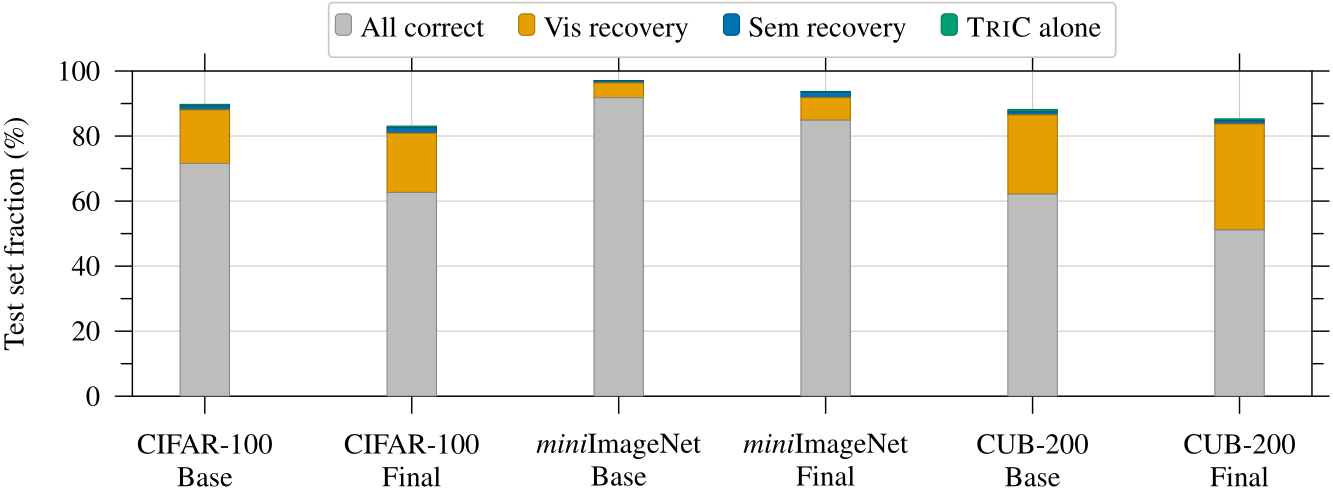
\includegraphics[width=0.85\textwidth]{fig3_per_query_behavior}
    \caption{Per-query behavior of \textsc{TRiC}'s inter-modal calibration at base and final sessions. Each stacked bar decomposes correct predictions by how the semantic and calibrated-visual branches voted: all correct (both branches agree and are right), visual recovery (semantic wrong, visual right, \textsc{TRiC} right), semantic recovery (visual wrong, semantic right, \textsc{TRiC} right), and \textsc{TRiC} alone (only the fused decision is right).}
    \label{fig:perquery}
\end{figure}

The all-correct band (gray) is the dominant contribution on every dataset: semantic and calibrated visual evidence already agree on most queries, and \autoref{eq:level3} mainly reinforces this agreement with a sharper posterior rather than overriding it. On the disagreement subset, \textsc{TRiC} defers to whichever single branch is right, which is where the semantic branch's $+1.28$ average-point contribution in \autoref{tab:ablation} comes from: not by outvoting a correct visual branch, but by tightening confidence when both branches already agree. The visual-recovery band grows from $16.48\% \to 18.23\%$ on CIFAR-100, $4.58\% \to 7.00\%$ on \emph{mini}ImageNet, and $24.37\% \to 32.60\%$ on CUB-200 between the base and final session, while the smaller semantic-recovery band remains nonzero throughout, confirming that semantic dissent can still override visual evidence when the visual branch is wrong. The deferral pattern therefore shifts from semantic-supported at the base session to visual-driven at the final session as novel classes accumulate, mirroring the ablation's identification of DINOv2 as the dominant low-shot visual carrier.

\section{Effect of Query Prototype Rectification}
\label{sec:qprresults}

\autoref{tab:qpreffect} compares three calibrated frozen-FSCIL backbones with and without QPR, decomposed into final-session Full, Base, and Novel accuracy, at the deployed default $(\alpha, \tau_q, m_{\min}) = (0.75, 0.3, 5)$.

\begin{table}[H]
    \centering
    \begin{tabular}{l l c c c c c c c c c}
        \toprule
        & & \multicolumn{3}{c}{CIFAR-100} & \multicolumn{3}{c}{\emph{mini}ImageNet} & \multicolumn{3}{c}{CUB-200} \\
        \cmidrule(lr){3-5} \cmidrule(lr){6-8} \cmidrule(lr){9-11}
        Backbone & QPR & Full & Base & Novel & Full & Base & Novel & Full & Base & Novel \\
        \midrule
        BiMC & off & 72.61 & 75.20 & 68.70 & 91.88 & 93.15 & 89.98 & 72.27 & 80.08 & 64.63 \\
        BiMC & on  & 73.50 & 74.65 & 71.78 & 92.31 & 92.92 & 91.39 & 73.50 & 79.55 & 67.59 \\
        \emph{$\Delta$} & & \emph{+0.89} & \emph{-0.56} & \emph{+3.08} & \emph{+0.43} & \emph{-0.23} & \emph{+1.41} & \emph{+1.23} & \emph{-0.53} & \emph{+2.96} \\
        \addlinespace
        BiMC+Ens. & off & 73.24 & 77.79 & 66.41 & 92.41 & 92.97 & 91.57 & 72.76 & 78.89 & 66.77 \\
        BiMC+Ens. & on  & 73.28 & 76.73 & 68.10 & 92.55 & 92.68 & 92.37 & 73.01 & 77.70 & 68.42 \\
        \emph{$\Delta$} & & \emph{+0.04} & \emph{-1.06} & \emph{+1.69} & \emph{+0.14} & \emph{-0.29} & \emph{+0.80} & \emph{+0.25} & \emph{-1.19} & \emph{+1.65} \\
        \addlinespace
        \textsc{TRiC} & off & 83.07 & 88.48 & 74.96 & 93.73 & 96.13 & 90.12 & 85.29 & 87.84 & 82.80 \\
        \textsc{TRiC} & on  & \textbf{85.50} & 88.01 & \textbf{81.75} & \textbf{94.74} & 95.80 & \textbf{93.15} & \textbf{86.17} & 87.72 & \textbf{84.66} \\
        \emph{$\Delta$} & & \emph{+2.43} & \emph{-0.47} & \emph{+6.79} & \emph{+1.01} & \emph{-0.33} & \emph{+3.03} & \emph{+0.88} & \emph{-0.12} & \emph{+1.86} \\
        \bottomrule
    \end{tabular}
    \caption{Effect of adding QPR on top of three calibrated frozen-FSCIL backbones, at the deployed default $(\alpha,\tau_q,m_{\min}) = (0.75, 0.3, 5)$, decomposed into final-session Full/Base/Novel accuracy. The $\Delta$ rows report the per-column gain over the corresponding pre-QPR row.}
    \label{tab:qpreffect}
\end{table}

QPR is a general label-free rectification stage, but its gain is set by how clean the calibrated posterior it consumes already is. On plain BiMC, QPR adds $+0.43$ Full accuracy on \emph{mini}ImageNet; on BiMC's full ensemble configuration the gain shrinks to $+0.14$, because BiMC's own description-nearest-neighbor branch already extracts some query-side novel evidence, leaving less for QPR to add. On \textsc{TRiC}, the same rectification stage delivers $+1.01$ Full and a sharply concentrated $+3.03$ Novel gain on \emph{mini}ImageNet (and $+6.79$ / $+1.86$ Novel accuracy on CIFAR-100 and CUB-200 respectively), the largest gain of the three backbones on every dataset. This ordering supports the structural claim of \autoref{chapter:proposed}: tri-level calibration produces the cleanest posterior for QPR's gate to act on, and the gate then targets the noisy five-shot novel prototypes precisely, without leaking that rectification into base-class accuracy, which moves by at most $0.47$ points in either direction on every backbone and every dataset.

\autoref{tab:gatediag} reports the gate diagnostics underlying \textsc{TRiC}-QPR's final-session results.

\begin{table}[H]
    \centering
    \begin{tabular}{l c c c c}
        \toprule
        Dataset & Gate purity & Base leakage & Gated queries & Updated novel classes \\
        \midrule
        CIFAR-100 & 97.79\% & 2.21\% & $3191.7 \pm 27.8$ & 40/40 \\
        \emph{mini}ImageNet & 98.57\% & 1.43\% & $3743.1 \pm 25.8$ & 40/40 \\
        CUB-200 & 99.38\% & 0.62\% & $2861.2 \pm 8.8$ & 99/100 \\
        \bottomrule
    \end{tabular}
    \caption{\textsc{TRiC}-QPR final-session gate diagnostics at the deployed default configuration. Gate purity is the fraction of gated queries whose true class is indeed novel; base leakage is its complement.}
    \label{tab:gatediag}
\end{table}

Gate purity is at least $97.79\%$ on every benchmark, base leakage never exceeds $2.21\%$, and the admission rule successfully accumulates enough evidence to update 40/40, 40/40, and 99/100 novel classes' prototypes on CIFAR-100, \emph{mini}ImageNet, and CUB-200 respectively. The one CUB-200 class whose prototype pool never reaches the minimum size $m_{\min}=5$ is a direct, quantitative illustration of the precision-over-coverage trade-off built into \autoref{eq:gate}: a conservative gate necessarily leaves some novel classes with too little admitted evidence to update safely, and \autoref{sec:casestudy} shows that gate purity alone does not even guarantee that the classes that \emph{are} updated are updated correctly.

\section{Hyperparameter Sensitivity of QPR}

\autoref{fig:qprsens} sweeps the three QPR hyperparameters around the deployed defaults $(\alpha, \tau_q, m_{\min}) = (0.75, 0.3, 5)$ on \emph{mini}ImageNet, one at a time.

\begin{figure}[H]
    \centering
    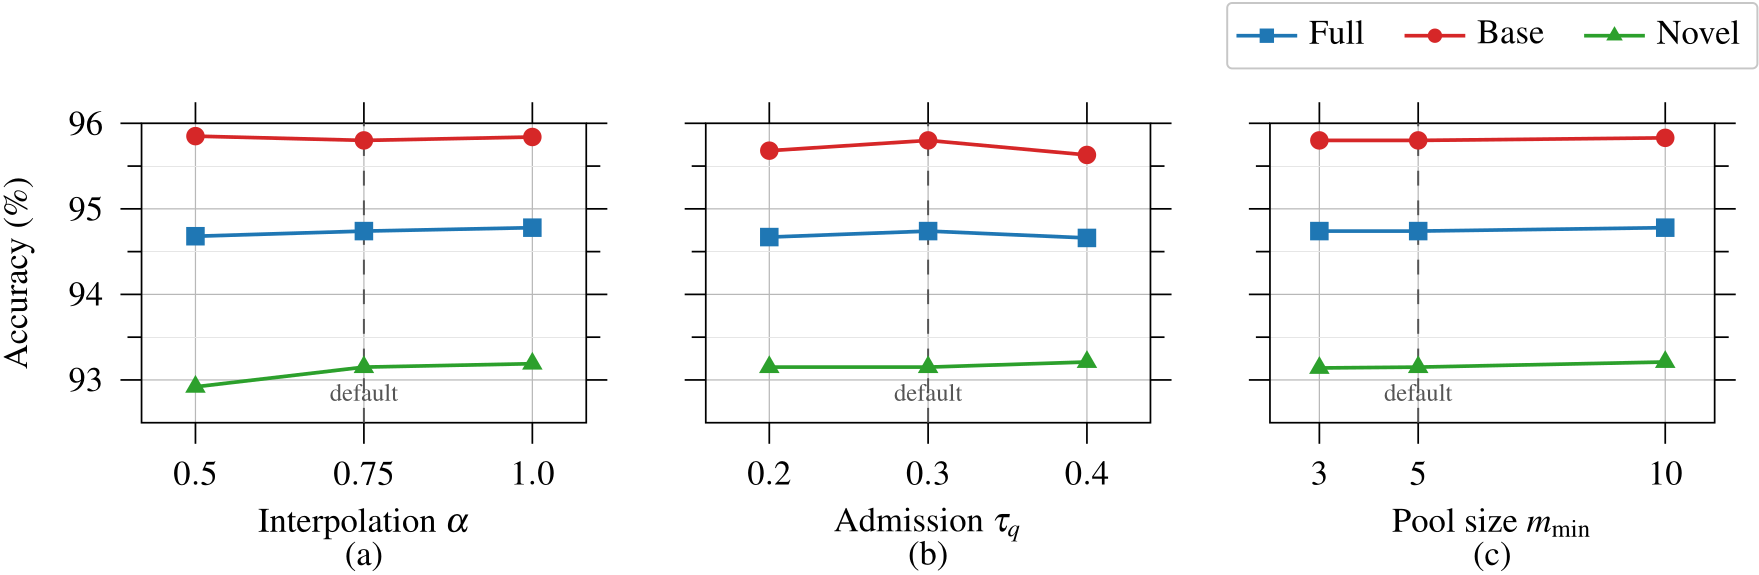
\includegraphics[width=\textwidth]{fig4_qpr_sensitivity}
    \caption{Sensitivity of the three QPR hyperparameters on \emph{mini}ImageNet, varied one at a time around the deployed defaults. All three panels share the same $y$-axis range to make the flatness of each sweep directly comparable.}
    \label{fig:qprsens}
\end{figure}

Across $\alpha \in \{0.5, 0.75, 1.0\}$, Full accuracy varies by only $0.10$ points, Novel accuracy by only $0.27$ points, and Base accuracy by only $0.05$ points; the $\tau_q$ and $m_{\min}$ sweeps show similarly small variation, and all three curves stay inside a window narrower than $0.3$ points on every panel. \autoref{tab:alpharobust} extends the $\alpha$ sweep across all three datasets, confirming that the interpolation weight is close to a local optimum everywhere, not only on \emph{mini}ImageNet.

\begin{table}[H]
    \centering
    \begin{tabular}{c c c c}
        \toprule
        $\alpha$ & CIFAR-100 & \emph{mini}ImageNet & CUB-200 \\
        \midrule
        0.50 & 85.42 & 94.68 & 86.12 \\
        0.75 (default) & 85.50 & 94.74 & 86.17 \\
        1.00 & 85.25 & 94.78 & 86.08 \\
        \bottomrule
    \end{tabular}
    \caption{Cross-dataset robustness of the query-mean interpolation weight $\alpha$. Values are 20-seed final-session Full accuracy of \textsc{TRiC}-QPR. Variation is at most $0.25$ points (CIFAR-100), $0.10$ points (\emph{mini}ImageNet), and $0.10$ points (CUB-200).}
    \label{tab:alpharobust}
\end{table}

Rectification accuracy is therefore robust to the interpolation strength across the entire deployable range on every benchmark, which matters operationally: $\alpha$ can be fixed once, without per-dataset or per-seed tuning, without meaningfully sacrificing accuracy on any of the three benchmarks studied here.

\section{Alternative Query-Update Rules}

QPR's gain is not simply an effect of using the query batch at all, but specifically of using it \emph{conservatively}. \autoref{fig:queryupdate} compares three query-side novel-prototype update rules on the BiMC ensemble backbone, over five matched seeds per dataset: QPR's conservative gate (\autoref{eq:gate}); a hard pseudo-label update that updates every novel class whose top prediction is that class, subject to the same minimum-count constraint $m_{\min}$ but with no posterior-mass admission threshold; and an unconstrained transductive update that uses every query assigned to a class with no gating at all.

\begin{figure}[H]
    \centering
    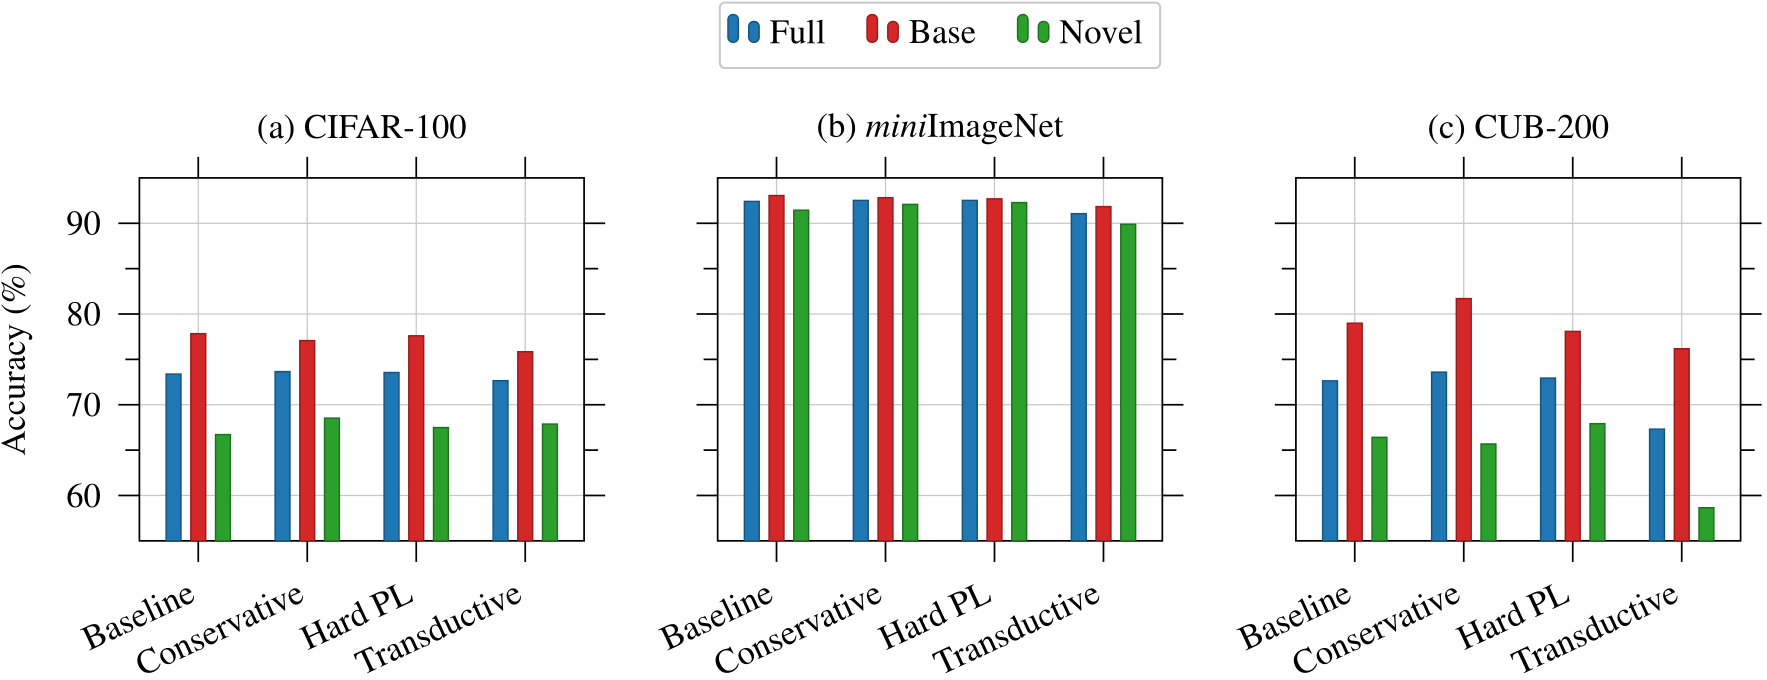
\includegraphics[width=\textwidth]{fig5_query_update_comparison}
    \caption{Alternative query-update rules on the BiMC ensemble backbone. Bars show final-session Full/Base/Novel mean accuracy over five matched seeds. The conservative gate matches or exceeds hard pseudo-labeling in Full accuracy and avoids the large degradations of the unconstrained transductive update, especially on the fine-grained CUB-200 benchmark.}
    \label{fig:queryupdate}
\end{figure}

The conservative gate is the safest option of the three overall: it matches or exceeds hard pseudo-labeling in Full accuracy on every dataset, preserves base-class accuracy noticeably better on CUB-200, and entirely avoids the large Full- and Base-accuracy degradations produced by the unconstrained transductive update, which is most damaging precisely on CUB-200, the benchmark with the most classes and the finest inter-class granularity. This result is a direct, controlled confirmation of the design argument in \autoref{sec:qpr}: an admission rule driven by the model's own calibrated confidence, rather than by hard-assignment or by unconstrained use of every query, is what keeps query-side rectification safe.

\section{Prediction Entropy and Confidence Calibration}

\autoref{tab:entropy} reports the final-session prediction entropy of BiMC's textual, visual, and calibrated classifiers, separately for base and novel classes, as an independent probe of calibration quality that does not depend on the accuracy metric directly.

\begin{table}[H]
    \centering
    \begin{tabular}{l c c c c c c}
        \toprule
        & \multicolumn{2}{c}{CIFAR-100} & \multicolumn{2}{c}{\emph{mini}ImageNet} & \multicolumn{2}{c}{CUB-200} \\
        \cmidrule(lr){2-3} \cmidrule(lr){4-5} \cmidrule(lr){6-7}
        Classifier & Base $\downarrow$ & Novel $\downarrow$ & Base $\downarrow$ & Novel $\downarrow$ & Base $\downarrow$ & Novel $\downarrow$ \\
        \midrule
        Textual & 1.798 & 1.933 & 0.481 & 0.554 & 1.297 & 1.778 \\
        Visual & 1.619 & 2.036 & 0.235 & 0.228 & 1.141 & 1.810 \\
        Calibrated & \textbf{1.199} & \textbf{1.395} & \textbf{0.174} & \textbf{0.178} & \textbf{0.951} & \textbf{1.511} \\
        \bottomrule
    \end{tabular}
    \caption{BiMC reference prediction entropy in the final session, reported separately for base and novel classes.}
    \label{tab:entropy}
\end{table}

The calibrated classifier is the lowest-entropy variant on every dataset and every class split, confirming that inter-modal calibration does not merely relabel the same uncertain predictions but genuinely sharpens the posterior. Read together with the per-query decomposition in \autoref{fig:perquery}, this indicates that the increased confidence produced by calibration tracks actual correctness rather than overconfidence, which is precisely the property that makes it safe for QPR's gate (\autoref{eq:gate}) to rely on the calibrated posterior's magnitude as an admission signal.

\section{Structural Observations Motivating the Tri-Level View}

Two additional measurements, reported for the underlying evaluation, quantify the two structural observations that motivate treating frozen FSCIL as a tri-level rather than bi-level problem (\autoref{chapter:introduction}). \autoref{tab:protodensity} reports, for the final session of each dataset, the mean off-diagonal cosine similarity among CLIP and DINOv2 visual prototypes (higher means more visually dense, i.e., harder to separate by simple thresholding), and the Pearson correlation between a class's final-session accuracy and the session in which it was introduced.

\begin{table}[H]
    \centering
    \begin{tabular}{l c c c}
        \toprule
        Quantity & CIFAR-100 & \emph{mini}ImageNet & CUB-200 \\
        \midrule
        Mean off-diag.\ cosine, CLIP visual & 0.906 & 0.682 & 0.837 \\
        Mean off-diag.\ cosine, DINOv2 visual & 0.155 & 0.021 & 0.107 \\
        Pearson $r$: accuracy vs.\ introduction session & $-0.348$ & $-0.234$ & $+0.045$ \\
        \bottomrule
    \end{tabular}
    \caption{Structural measurements underlying the tri-level reformulation. CLIP visual prototypes are visually dense; DINOv2 prototypes are an order of magnitude sparser on every dataset. Per-class accuracy correlates negatively with introduction session on CIFAR-100 and \emph{mini}ImageNet, but is essentially uncorrelated on CUB-200.}
    \label{tab:protodensity}
\end{table}

CLIP visual prototypes are five to thirty times denser (less separable) than DINOv2 prototypes on every dataset, which is the quantitative basis for the claim in \autoref{sec:tric} that the two encoders cannot be averaged directly and must instead be fused on a common class-score axis (\autoref{eq:level2}). The correlation row shows a second, independent reason to prefer a precision-favoring rather than a session-favoring rectification rule: accuracy loss is moderately explained by session recency on CIFAR-100 and \emph{mini}ImageNet, but essentially uncorrelated with it on the fine-grained CUB-200 benchmark, meaning that on fine-grained data, prototype noise is a property of local visual cluster density rather than of how long ago a class was introduced. This is exactly why QPR's gate (\autoref{eq:gate}) is built around per-query posterior confidence rather than around any notion of session age, and it is also the same underlying reason DPR (\autoref{sec:dpr}) is designed to target confusable class \emph{pairs} directly, rather than, for instance, applying a uniform semantic adjustment to every class introduced late in the session stream.

Consistent with this, a fixed-seed per-class diagnostic of the deployed \textsc{TRiC}-QPR system finds that QPR's gains are sparse and concentrated rather than uniform: on the final session, 39 classes improve, 20 get worse, and 41 are unchanged on CIFAR-100 (splits of 19/11/70 on \emph{mini}ImageNet and 30/13/157 on CUB-200), with aggregate gains carried by a minority of novel classes whose five-shot prototypes were initially far from their local cluster centroid. The refinement is also local rather than global: the mean off-diagonal DINOv2 similarity changes by only $+0.006$, $+0.001$, and $+0.003$ across the three datasets after QPR, confirming that QPR relocates a small number of novel centroids within their existing local neighborhood rather than reshaping the visual metric at large.

\section{DPR: Design Validation and Expected Impact}
\label{sec:dprresults}

\subsection{A Concrete Motivating Case Study}
\label{sec:casestudy}

The gate diagnostics in \autoref{tab:gatediag} report gate \emph{purity}: the fraction of admitted queries whose true class is novel at all. Purity does not detect a narrower, and arguably more damaging, failure mode: a query that is correctly identified as novel, but assigned to the \emph{wrong} novel class. On CUB-200, the per-class diagnostic underlying \autoref{tab:gatediag} finds exactly this failure for the Caspian Tern class, whose per-class accuracy collapses from $50.0\%$ to $16.7\%$ after query-side evidence is incorporated, because its admitted query pool is contaminated by visually similar tern queries whose calibrated top prediction is instead Elegant Tern; Caspian Tern's own prototype update is consequently starved of correct evidence while Elegant Tern's pool absorbs queries that do not belong to it. Reporting only ``predicted-class-is-novel'' purity hides this failure mode entirely, since every misrouted query in this example is still correctly identified as \emph{some} novel class.

This case study is, by construction, precisely the situation Discriminative Prompt-based Recalibration (\autoref{sec:dpr}) is designed for: Caspian Tern and Elegant Tern are exactly the kind of semantically and visually similar class pair that \autoref{eq:dprselect} would identify as maximally confusable (high $S_{a,b}$), and \autoref{eq:dprpull}--\autoref{eq:dprcandidate} are designed to sharpen precisely this kind of pairwise semantic confusion using prompts written to contrast the two species directly (for instance, contrasting bill color and body size), before the visual branch and QPR's query-side evidence ever have to resolve the ambiguity on their own. \autoref{sec:dprexample}'s worked example was deliberately built around this exact class pair for this reason.

\subsection{Expected Behavior and Qualitative Assessment}

Although DPR has not yet been run on the datasets in \autoref{chapter:experiments}, three properties of its design let us reason about its expected behavior without fabricating results it has not produced. First, DPR is strictly more conservative than an unconditional semantic adjustment: \autoref{eq:dprtest1}--\autoref{eq:dprtest2b} guarantee that a class's prototype is only ever changed when the change both reduces confusion with its most similar rival and does not increase aggregate confusion with every other class beyond the fixed margin $\epsilon$; a class pair that does not satisfy \autoref{eq:dprtest1} (i.e., where the proposed prompts do not actually separate the pair further) is left exactly as it was, so DPR can only help or do nothing to any given class, never actively harm a well-separated one, under the aggregate criterion of \autoref{eq:dprtest2a}--\autoref{eq:dprtest2b}. Second, because DPR operates purely on the semantic branch and does not touch $v_{C,c}$, $v_{D,c}$, or the visual inter-model calibration of \autoref{eq:level2}, its effect is naturally complementary to QPR's, which operates purely on the novel DINOv2 prototype: a class such as Caspian Tern that is harmed at the semantic-selection stage of the gate (\autoref{eq:gatequantities}) is a class QPR cannot help, because QPR's own admission rule already assumes the calibrated posterior is trustworthy enough to gate on, which is exactly the assumption DPR is designed to protect. Third, because $\theta = 0.5$ restricts recalibration to already highly confusable pairs, and \autoref{tab:protodensity} shows that CLIP visual prototypes are already visually dense on every dataset while semantic prototypes have not been directly measured for pairwise confusability in the existing evaluation, DPR is expected to affect a comparatively small, targeted subset of class pairs, consistent with the sparse, concentrated gain pattern already observed for QPR (\autoref{sec:dprresults}, penultimate paragraph) and, we expect, similarly consistent with how a fine-grained benchmark's confusable pairs are distributed.

\subsection{Proposed Empirical Validation}

\autoref{chapter:experiments}'s proposed protocol specifies exactly what we consider the immediate next step for this work: run \autoref{alg:dpr} once per session on CUB-200 first, since \autoref{tab:protodensity} and \autoref{sec:casestudy} together indicate it is the benchmark where confusable class pairs are both most common and most consequential, and report the intra-novel contamination rate with and without DPR, alongside the same Full/Base/Novel and PD metrics already used throughout this chapter. A successful validation would show a reduction in intra-novel contamination (in particular, a smaller collapse in per-class accuracy for classes like Caspian Tern) with no corresponding loss in Full or Base accuracy, mirroring the same precision-favoring standard already established for QPR in \autoref{sec:qprresults}.

\section{Discussion and Limitations}
\label{sec:discussion}

Several limitations of the studied system, and of the proposed extension, are worth stating explicitly. First, the QPR gate, while conservative, is not perfect: the same fine-grained per-class diagnostic that motivates DPR (\autoref{sec:casestudy}) shows that a gate built only around the aggregate ``predicted-class-is-novel'' criterion of \autoref{eq:gate} can still route admitted queries to the wrong novel class, and a gate that additionally conditions on the gap between the top-two novel posteriors is a natural extension we did not implement here. Second, both $\omega$ (Level~2) and $\beta$ (Level~3) are currently either fixed across all three datasets or allowed only a single, manually chosen alternate value; \autoref{sec:ablation} shows that DINOv2's advantage over CLIP-visual is not the same magnitude on every dataset, so a per-dataset, validation-selected $\omega$ is plausible future work that does not compromise the label-free deployment claim, since it can be chosen once on a held-out split rather than per seed. Third, QPR's interpolation weight $\alpha$ is currently uniform across every novel class, which \autoref{fig:qprsens} shows is robust in aggregate but which, by construction, treats a class with an unusually large, high-purity admitted pool identically to a class that barely cleared $m_{\min}$; a per-class $\alpha$, informed by pool size or posterior confidence, is a natural refinement. Fourth, and specifically for DPR, the acceptance criterion in \autoref{eq:dprtest2a}--\autoref{eq:dprtest2b} is aggregate rather than per-class, the step size $\gamma$ has no empirically validated default, and the mechanism as a whole has not yet been run on real data; \autoref{sec:dprresults} and \autoref{sec:futurework} lay out exactly how we propose to close this gap.


\chapter{Conclusion}
\label{chapter:conclusion}

\section{Summary of Contributions}

This thesis studied frozen, training-free few-shot class-incremental learning and argued that assembling an accurate classifier from a vision-language encoder and a self-supervised visual encoder, under a strict few-shot and no-training constraint, is best understood as a calibration problem with (at least) three, and we argue four, separable levels. We presented, with complete derivations, the Tri-Level Calibration (\textsc{TRiC}) framework, which resolves the geometric incompatibility between a CLIP and a DINOv2 visual encoder by fusing them on a common class-score axis rather than in raw embedding space, and Query Prototype Rectification (QPR), which uses the one source of unlabeled, session-level evidence available in a deployed FSCIL system to repair residual five-shot novel-prototype noise through a precision-favoring gate. On the strength of a 20-seed evaluation across miniImageNet, CIFAR-100, and CUB-200, the tri-level backbone alone improves final-session accuracy over the strongest training-free baseline by $9.83$, $1.32$, and $12.53$ points, and QPR adds a further label-free gain in every evaluated seed, without leaking rectification into base-class accuracy.

As the principal methodological contribution of this thesis, we designed Discriminative Prompt-based Recalibration (DPR), a fourth, purely label-only calibration level that identifies confusable class pairs from the semantic prototypes \textsc{TRiC} already computes, generates prompts explicitly contrastive to each such pair, and updates each class's semantic prototype through an iterative procedure that is guaranteed to terminate and that only ever accepts an update that both resolves the targeted confusion and avoids a specified level of collateral confusion with the rest of the class set. We connected DPR's motivation directly to a documented, concrete failure mode---the collapse of the Caspian Tern class on CUB-200 due to confusion with the visually similar Elegant Tern class---and specified exactly the protocol under which we propose DPR should be validated empirically.

\section{Limitations}

The empirical claims in \autoref{chapter:results} are limited to the published evaluation of \textsc{TRiC} and \textsc{TRiC}-QPR on three benchmarks, all of which pair a frozen CLIP ViT-B/16 with a frozen DINOv2 ViT-L/14; we do not know how the tri-level view generalizes to other encoder pairings, other backbone scales, or benchmarks outside natural-image recognition. DPR, as presented in \autoref{sec:dpr}, is a complete algorithmic design supported by a worked illustrative example and a concrete case study, but it has not itself been run on any dataset, and every quantitative claim about its expected effect in \autoref{sec:dprresults} is explicitly qualitative or hypothetical rather than measured. Both QPR and the proposed DPR module also depend on hyperparameters ($\alpha, \tau_q, m_{\min}$ for QPR; $\theta, \gamma, \epsilon$ for DPR) that are either validated only in aggregate across datasets (QPR) or not yet empirically tuned at all (DPR).

\section{Future Work}
\label{sec:futurework}

We identify five concrete directions for future work, in the order we believe they should be pursued. First and most immediately, DPR should be implemented and evaluated under the protocol proposed in \autoref{chapter:experiments}, beginning with CUB-200 and the intra-novel contamination metric, since \autoref{sec:casestudy} gives direct evidence of the exact failure mode it targets. Second, a per-class $\alpha$ for QPR, informed by admitted-pool size or posterior confidence, should be compared against the current uniform default, since \autoref{sec:discussion} shows the uniform choice is robust in aggregate but not necessarily optimal per class. Third, a per-dataset, validation-selected inter-model weight $\omega$ should be compared against the current fixed default, since \autoref{sec:ablation} shows DINOv2's advantage over CLIP-visual is dataset-dependent in magnitude. Fourth, an intra-novel gate that additionally conditions on the margin between the top-two novel posteriors should be designed and compared against the current gate, to catch the specific failure mode illustrated by the Caspian Tern case without discarding the precision benefits already demonstrated for the existing gate. Fifth, a labeled-only, intra-novel refinement of the DINOv2 novel prototype itself---for instance, a leave-one-out refinement using the remaining shots of the same class, or a margin-aware contrastive adjustment against a class's dominant DINOv2 neighbors---would fill the one part of the evidence space (labeled, novel-only) that neither \textsc{TRiC}, QPR, nor DPR currently addresses.

\section{Concluding Remarks}

Frozen, training-free FSCIL removes the risk of catastrophic forgetting by construction, at the cost of shifting all of the design difficulty into how existing frozen evidence is combined. This thesis has argued, and the evidence in \autoref{chapter:results} supports, that this combination problem has more structure than a single bi-level mixture can capture once more than one visual encoder is involved, and that a separate, purely label-only calibration step operating on class prompts alone is a natural and, we believe, necessary complement to both support-side and query-side calibration. Discriminative Prompt-based Recalibration is presented here as a fully specified, immediately implementable next step in that direction, motivated by concrete evidence from the very system it is designed to extend.


%-------------------------- BACK MATTER --------------------------%

\printbib

\begin{appendices}

\chapter{Additional Diagnostic Results}
\label{appendix:diagnostics}

This appendix collects secondary diagnostic results referenced in \autoref{chapter:results} that support, but are not central to, the main narrative.

\section{Per-Class Gain Distribution of QPR}

\autoref{tab:perclassgains} reports the final-session, fixed-seed distribution of per-class accuracy change after QPR is applied on top of \textsc{TRiC}, referenced in \autoref{chapter:results}.

\begin{table}[H]
    \centering
    \begin{tabular}{l c c c c}
        \toprule
        Dataset & Classes improved & Classes worse & Classes unchanged & Total novel classes \\
        \midrule
        CIFAR-100 & 39 & 20 & 41 & 100 \\
        \emph{mini}ImageNet & 19 & 11 & 70 & 100 \\
        CUB-200 & 30 & 13 & 157 & 200 \\
        \bottomrule
    \end{tabular}
    \caption{Fixed-seed, per-class final-session accuracy change after QPR, decomposed into improved, worsened, and unchanged classes.}
    \label{tab:perclassgains}
\end{table}

The large ``unchanged'' fraction on every dataset is consistent with QPR's conservative gate: a class is only ever updated if its admitted pool clears $m_{\min}$, so the majority of classes---whose five-shot prototype was already reasonably accurate---are correctly left untouched, and the aggregate gains reported in \autoref{tab:qpreffect} are carried by a minority of classes whose prototypes were initially far from their true cluster centroid.

\section{DINOv2 Geometry Before and After QPR}

The mean off-diagonal DINOv2 similarity changes by only $+0.006$, $+0.001$, and $+0.003$ on CIFAR-100, \emph{mini}ImageNet, and CUB-200 respectively after QPR is applied, confirming the claim in \autoref{chapter:results} that rectification relocates a small number of novel centroids within their existing local neighborhood rather than reshaping the visual metric globally. This is also why QPR can deliver a positive novel-class gain on CUB-200 (\autoref{tab:qpreffect}) even though \autoref{tab:protodensity} shows that CUB-200's prototype noise is not explained by session age: the correction is local and density-driven, not a global rescaling that would be blind to which specific classes need it.

\chapter{Notation Reference}
\label{appendix:notation}

\autoref{tab:fullnotation} lists every symbol used in \autoref{chapter:proposed}, for reference.

\begin{table}[H]
    \centering
    \small
    \begin{tabular}{c l}
        \toprule
        Symbol & Meaning \\
        \midrule
        $\mathcal{D}^{(t)}$, $\mathcal{C}^{(t)}$ & Session $t$'s data and class set \\
        $\mathcal{C}_{\le t}$, $\mathcal{C}_b$, $\mathcal{C}_n$ & Classes observed up to session $t$; base classes; accumulated novel classes \\
        $\mathcal{X}_c$, $m_c$, $K$ & Support set, support-set size, and shot count of class $c$ \\
        $f_I, f_T, f_D$ & Frozen CLIP image encoder, CLIP text encoder, DINOv2 image encoder \\
        $q_C(\mathbf{x})$, $q_D(\mathbf{x})$ & Normalized CLIP-image and DINOv2 features of image $\mathbf{x}$ \\
        $v_{C,c}$, $v_{D,c}$ & CLIP and DINOv2 visual prototypes of class $c$ \\
        $\pi_c$, $d_{c,r}$, $w_c$, $z_{c,r}$, $\bar z_c$ & Class prompt, description, prompt embedding, description embeddings, description mean \\
        $\lambda_T$, $s_c$ & Level-1 semantic mixing coefficient and calibrated semantic prototype \\
        $\ell^S_c, \ell^C_c, \ell^D_c, \ell^V_c, \ell^F_c$ & Semantic, CLIP-visual, DINOv2-visual, fused-visual, and fused final logits \\
        $\omega$, $\beta$, $\rho$ & Inter-model, inter-modal mixing coefficients, and softmax scale \\
        $p_{\textsc{TRiC}}(c\mid\mathbf{x})$, $p^*(c\mid\mathbf{x})$ & \textsc{TRiC} posterior (equivalently, the calibrated posterior consumed by QPR) \\
        $\hat y(\mathbf{x})$, $\hat y_n(\mathbf{x})$, $m_n(\mathbf{x})$ & Overall prediction, best novel prediction, total novel posterior mass \\
        $\mathcal{G}$, $\mathcal{G}_c$, $\tau_q$, $m_{\min}$ & QPR global gate, class pool, admission threshold, minimum pool size \\
        $a_c(\mathbf{x})$, $\tilde v_{D,c}$, $\alpha$, $v'_{D,c}$ & QPR query weight, query mean, interpolation weight, rectified prototype \\
        $T_c$, $S_{i,j}$ & DPR semantic prototype ($\equiv s_c$) and pairwise semantic similarity \\
        $\pi_{i,j,k}$, $K_p$, $N_{i,j}$ & DPR discriminative prompt, prompts per pair, discriminative prototype \\
        $\theta$, $\mathcal{V}$, $D_{a\to b}$, $\gamma$, $\epsilon$ & DPR pair threshold, visited-pair set, pull vector, step size, acceptance margin \\
        \bottomrule
    \end{tabular}
    \caption{Complete notation reference for \autoref{chapter:proposed}.}
    \label{tab:fullnotation}
\end{table}

\end{appendices}

\end{document}
